\documentclass[a4paper,12pt, PhD]{stb-thesis}

% Imports
% Page layout
\usepackage[left=3cm,right=2cm,top=2.5cm,bottom=2.5cm]{geometry}
%\usepackage{cite}
\usepackage{afterpage}
\newcommand\blankpage{%
	\null
	\thispagestyle{empty}%
	\addtocounter{page}{-1}%
	\newpage}

% Subsections
\setcounter{secnumdepth}{3}
\setcounter{tocdepth}{3}

% Figures
\usepackage[margin=\the\parindent,small,bf,rm]{caption}
\usepackage{graphicx}
\usepackage{pdfpages}
\setlength{\abovecaptionskip}{8pt}  % spacing above and below captions
\usepackage{subfig}
\usepackage{svg}
\usepackage{float}

% Font and text
\usepackage[afrikaans,english]{babel}
\usepackage{microtype}
\usepackage{setspace}
\newcommand{\myemph}[1]{{\sffamily\bfseries#1}}
\sloppy
\onehalfspacing
\usepackage{enumitem}
%\setlist[enumerate]{noitemsep, topsep=0pt, partopsep=0pt}
\usepackage{listings,xfp}
\usepackage{anyfontsize}
\usepackage{bold-extra}
\usepackage{quotchap}

\renewcommand\labelitemi{\tinytonormal$\divideontimes$}

\makeatletter
{\large % Capture font definitions of \small
	\xdef\f@size@large{\f@size}
	\xdef\f@baselineskip@large{\f@baselineskip}
	\Large % Capture font definitions for \normalsize
	\xdef\f@size@Large{\f@size}
	\xdef\f@baselineskip@Large{\f@baselineskip}
}
% Define new \smalltonormalsize font size
\newcommand{\largetoLarge}{%
	\fontsize
	{\fpeval{(\f@size@large+\f@size@Large)/2}}
	{\fpeval{(\f@baselineskip@large+\f@baselineskip@Large)/2}}%
	\selectfont
}
\makeatother
\makeatletter
{\tiny % Capture font definitions of \small
	\xdef\f@size@tiny{\f@size}
	\xdef\f@baselineskip@tiny{\f@baselineskip}
	\normalsize % Capture font definitions for \normalsize
	\xdef\f@size@normalsize{\f@size}
	\xdef\f@baselineskip@normalsize{\f@baselineskip}
}
% Define new \smalltonormalsize font size
\newcommand{\tinytonormal}{%
	\fontsize
	{\fpeval{(\f@size@tiny+\f@size@normalsize)/2}}
	{\fpeval{(\f@baselineskip@tiny+\f@baselineskip@normalsize)/2}}%
	\selectfont
}
\makeatother
\makeatletter
{\tiny % Capture font definitions of \small
	\xdef\f@size@tiny{\f@size}
	\xdef\f@baselineskip@tiny{\f@baselineskip}
	\normalsize % Capture font definitions for \normalsize
	\xdef\f@size@normalsize{\f@size}
	\xdef\f@baselineskip@normalsize{\f@baselineskip}
}
% Define new \smalltonormalsize font size
\newcommand{\othertinytonormal}{%
	\fontsize
	{\fpeval{(\f@size@tiny+\f@size@normalsize)*0.4}}
	{\fpeval{(\f@baselineskip@tiny+\f@baselineskip@normalsize)*0.4}}%
	\selectfont
}
\makeatother

% Headings
\usepackage{textcase}
\usepackage{mfirstuc}
\usepackage{titlecaps}
\usepackage{stringstrings}
\usepackage[raggedright,rm,bf]{titlesec}
\usepackage{titlecaps}
\titlelabel{\thetitle.\quad}
\titleformat{\chapter}[display]{\LARGE\rmfamily\raggedleft}{\scshape \chaptertitlename\ \thechapter}{3pt}{\titlerule\vspace{1.5ex} \scshape \Huge \centering}[\vspace{1.5ex}\titlerule]
\titlespacing*{\chapter}{0pt}{30pt}{40pt}  % remove spacing before chapter headings

\titleformat{\section}{\rmfamily\scshape\Large}{\thesection}{1em}{}
\titleformat{\subsection}{\rmfamily\scshape\large}{\thesubsection}{1em}{}
\titleformat{\subsubsection}{\rmfamily\scshape\normalsize}{\thesubsubsection}{1em}{}

\newcommand{\ShortInTextTitle}[1]{\textbf{\scshape #1}}

% Table of contents
\usepackage{xcolor,titletoc}
\makeatletter
\let\originall@chapter\l@chapter
\def\l@chapter#1#2{\originall@chapter{{\rmfamily #1}}{#2}}
\makeatother
\let \savenumberline \numberline
\def \numberline#1{\savenumberline{#1.}}

% Nomenclaure
\usepackage{acro}
\usepackage{multicol}
%\usepackage{scrextend}
\usepackage{ragged2e}
\newlength\myitemwidth
\setlength\myitemwidth{5cm}
\newlist{myacronymlist}{description}{1}
\setlist[myacronymlist]{
	%	itemsep = 1000pt,
	labelindent = 0pt ,
	labelsep    = 0pt ,
	leftmargin  = \myitemwidth ,
	labelwidth  = \myitemwidth ,
	itemindent  = 0pt ,
	format      = \RaggedRight 
}
%\NewAcroTemplate[list]{styleabbrev}{%
	%	\UseAcroTemplate[list]{description}[0]%
	%}
%\NewAcroTemplate[list]{styleabbrev}{%
	%		\UseAcroTemplate[list]{myacronymlist}[0]%
	%		\acropreamble
	%		\begin{itemize}
		%			\acronymsmapF
		%			{\item[\bfseries\acrowrite{short}] \acrowrite{alt}}
		%			{\item\AcroRerun}
		%		\end{itemize}
	%}
\RenewAcroTemplate{long-short}{%
	\acroiffirstTF{%
		\acrowrite{long}%
		\acspace(%
		\acroifT{foreign}{\acrowrite{foreign}, }%
		\acrowrite{short}%
		\acroifT{alt}{}%
		\acrogroupcite
		)%
	}%
	{\acrowrite{short}}%
}
\NewAcroTemplate[list]{styleabbrev}{%
	\normalsize
	\AcroNeedPackage{array}%
	\acronymsmapF{
		\AcroAddRow{
			\vspace{1.0ex}\par
			\acrowrite{short} & \acrowrite{alt}
			\acropagefill
			\acropages
			{\acrotranslate{page}\nobreakspace}
			{\acrotranslate{pages}\nobreakspace}%
			\tabularnewline
			% 			\vspace{1.8ex}\par
		}%
	}
	{\AcroRerun}%
	%    \acroheading
	\acropreamble
	\par\noindent
	\begin{tabular}{>{\bfseries}lp{.7\linewidth}}
		\AcronymTable
	\end{tabular}
}

\acsetup{
	list/template  = styleabbrev,
	%	list/display=used,
	%	list/sort=true,
	%	format=\RaggedRight
}

\usepackage[toc,section=section,nonumberlist]{glossaries-extra}
\usepackage{glossary-superragged}
\usepackage[intoc, english]{nomencl}
\usepackage{tabularx, booktabs}
\usepackage{calc}

\newlength{\mycolwidth}

%\newglossarystyle{mystyle}{
	%	\setglossarystyle{treegroup}%
	%	\renewcommand*{\glossentry}[2]{%
		%		\glsentryitem{##1}%
		%		\settowidth{\mycolwidth}{{\textsc{\mdseries\glossentryname{##1}} }}%
		%		\begin{tabular}{@{} l p{\dimexpr\textwidth-\mycolwidth\relax} @{}}
			%			{\textsc{\mdseries\glossentryname{##1}} }& \glossentrydesc{##1}\\
			%		\end{tabular}%
		%		\par\vspace{10pt}
		%	}
	%}
\newglossarystyle{mystyle}{
	\setglossarystyle{treegroup}%
	\renewcommand*{\glossentry}[2]{%
		\glsentryitem{##1}%
		%		\settowidth{\mycolwidth}{{\textsc{\mdseries\glossentryname{##1}} }}%
		{\textsc{\textbf{\glossentryname{##1}}}}
		\glossentrydesc{##1}
		\vspace{10pt}
		
	}
}
%\renewcommand{\glsnamefont}[1]{\textsc{\mdseries #1}}
\setglossarystyle{mystyle}

\renewcommand{\nomgroup}[1]{%
	\ifthenelse{\equal{#1}{V}}{\item[{\rmfamily\scshape\Large Variables}]}{%
		\ifthenelse{\equal{#1}{C}}{\item[{\rmfamily\scshape\Large Constants}]}{
			\ifthenelse{\equal{#1}{F}}{\item[{\rmfamily\scshape\Large Functions}]}{}}}%
}

\makenomenclature
\newcommand{\altnomname}{\nomname}
\makeatletter
\def\thenomenclature{%
    \section*{\nomname}
    \vspace{10pt}
    \if@intoc\addcontentsline{toc}{section}{\altnomname}\fi%

  \nompreamble
  \list{}{%
    \labelwidth\nom@tempdim
    \leftmargin\labelwidth
    \advance\leftmargin\labelsep
    \itemsep\nomitemsep
    \let\makelabel\nomlabel}}
\makeatother

\makeatletter
\renewcommand\tableofcontents{%
	\chapter*{\contentsname}%
	\@mkboth{\scshape \contentsname}%
	{\scshape \contentsname}%
	\@starttoc{toc}%
}
\renewcommand\listoftables{%
	\chapter*{\listtablename}%
	\@mkboth{\scshape\listtablename}%
	{\scshape\listtablename}%
	\@starttoc{lot}%
}
\renewcommand\listoffigures{%
	\chapter*{\listfigurename}%
	\@mkboth{\scshape\listfigurename}%
	{\scshape\listfigurename}%
	\@starttoc{lof}%
}
\makeatother


% Mathematics
%\usepackage[cmex10]{amsmath}
\usepackage{amssymb}
\usepackage{cancel}
\DeclareMathOperator*{\argmax}{arg\,max}
\newcommand{\T}{^\textrm{T}}
\newcommand{\tr}{\textrm{tr}}
\newcommand{\defeq}{\triangleq}

% Tables
\usepackage{placeins}
\usepackage{array}
\usepackage{colortbl}
\usepackage{longtable}
\usepackage{ltcaption}
%\renewcommand\LTcaptype{figure}
\usepackage{multirow}
\newcommand{\mytable}{
	\centering
	\small
	%     \renewcommand{\arraystretch}{1.2}
	\renewcommand{\arraystretch}{1.2}
}
\renewcommand{\tabularxcolumn}[1]{m{#1}}
\newcommand{\PreserveBackslash}[1]{\let\temp=\\#1\let\\=\temp}
\newcolumntype{C}{>{\centering\arraybackslash}X}
\newcolumntype{L}{>{\raggedright\arraybackslash}X}
\newcolumntype{A}[1]{>{\PreserveBackslash\raggedright}p{#1}}
\renewcommand{\topfraction}{.60}
\renewcommand{\bottomfraction}{.85}
\renewcommand{\textfraction}{.05}
\renewcommand{\floatpagefraction}{.66}
\renewcommand{\dbltopfraction}{.66}
\renewcommand{\dblfloatpagefraction}{.66}
\setcounter{topnumber}{2}
\setcounter{bottomnumber}{9}
\setcounter{totalnumber}{20}
\setcounter{dbltopnumber}{2}

% Descriptions
\usepackage[T1]{fontenc}
\usepackage{lmodern} % To switch to Latin Modern
\rmfamily % To load Latin Modern Roman and enable the following NFSS declarations.
% Declare that Latin Modern Roman (lmr) should take
% its bold (b) and bold extended (bx) weight, and small capital (sc) shape, 
% from the corresponding Computer Modern Roman (cmr) font, for the T1 font encoding.
\DeclareFontShape{T1}{lmr}{b}{sc}{<->ssub*cmr/bx/sc}{}
\DeclareFontShape{T1}{lmr}{bx}{sc}{<->ssub*cmr/bx/sc}{}
\setlist[description]{ 
	labelwidth=0.6\textwidth,%
	leftmargin=\labelwidth, 
	align=right,
	font=\normalfont\scshape\bfseries
}
\newcommand{\mydefinition}[2] {
	\begin{flushright}
		\textbf{\textsc{#1}} #2 \\
	\end{flushright}
}

\usepackage{makecell}
\usepackage{mdframed}
\newcommand{\defblock}[3]{
	\begin{mdframed}[roundcorner=100pt]
		\begin{tabular}{@{}lp{#3ex}@{}}
			\textbf{\textsc{#1}}: & #2
		\end{tabular}
	\end{mdframed}
}

\usepackage{environ}
\usepackage{tikz}
\usetikzlibrary{fit,backgrounds,calc}
% Pseudo-code
\usepackage{algorithm}  % should go before \usepackage{hyperref}
\NewEnviron{defbox}[3]
{
	%	\begin{tikzpicture}
		%		\node[inner sep=0pt,
		%		draw=cambrigeblue,
		%		line width=1.2pt,
		%		rounded corners=0.25cm] (box) {\parbox[t]{\textwidth}
			%			{
				\vspace{15pt}\\
				\begin{tabular}{@{}lp{#3ex}@{}}
					\RaggedLeft{\textbf{\textsc{#1}}:} & #2
				\end{tabular}
				\vspace{15pt}\\
				%			}%
			%		};
		%		
		%	\end{tikzpicture}
}


% Table of contents and hyperlinks
\usepackage[linktocpage=true]{hyperref}
%\hypersetup{colorlinks=true,linktoc=all,allcolors=gray!80!black}
\hypersetup{
	colorlinks=true,
	linktoc=all,
	linkcolor=black, 
	filecolor=black, 
	citecolor = gray!80!black,       
	urlcolor=gray!80!black,
}
%\usepackage[nottoc,notlot,notlof]{tocbibind}
 \usepackage{url}
\usepackage{blindtext}

% Pseudo-code
\usepackage{algpseudocode}  % should go after \usepackage{hyperref}
%\renewcommand{\thealgorithm}{\arabic{chapter}.\arabic{algorithm}} 
%\captionsetup[algorithm]{labelfont={bf},font=small,labelsep=colon}

% Fix titlesec issue
\usepackage{etoolbox}
\makeatletter
\patchcmd{\ttlh@hang}{\parindent\z@}{\parindent\z@\leavevmode}{}{}
\patchcmd{\ttlh@hang}{\noindent}{}{}{}
\makeatother

% Bibliography
% \usepackage[round]{natbib}
\usepackage[square,numbers,compress,sort]{natbib}
\bibliographystyle{IEEEtranN}
% \usepackage[round]{natbib}
%\bibliographystyle{apalike}
%\usepackage{cite}
\usepackage{bibentry}
\nobibliography*

% Header and footer
\newcommand{\listheaderfont}{\scshape}
%\renewcommand{\tocetcmark}[1]{
	%	\markboth{\listheaderfont #1}{\listheaderfont #1}}
\usepackage{fancyhdr}
\usepackage{extramarks}
\pagestyle{fancy}
\fancyhf{}
\renewcommand{\chaptermark}[1]{\markboth{\normalsize \rmfamily \thechapter.\ \scshape #1}{\normalsize \rmfamily \thechapter.\ \scshape #1}}
\renewcommand{\sectionmark}[1]{\markright{\normalsize \rmfamily \thesection.\ \scshape #1}}
%\renewcommand{\sectionmark}[1]{\markright{\normalsize \rmfamily \thesection.\ \scshape #1}{}}
\fancyhead[C]{\color{oraclecolor} \rightmark \\ \color{rulecolor} \rule{\textwidth}{0.1pt}}
\fancyfoot{}
\fancyfoot[R]{\thepage}{}

% \setlength\headheight{14.5pt}
\setlength{\headheight}{27.11653pt}
\renewcommand{\headrulewidth}{0pt}
\fancypagestyle{plain}{\fancyhead{}
	\renewcommand{\headrulewidth}{0pt}
	%	\fancyfoot[C]{\thepage}
}

\newcommand{\mysubsubsection}[2]{
	%	\sectionmark{#2}
	\let\orisubsubsectionmark\subsubsectionmark
	\renewcommand\subsubsectionmark[1]{}%
	\subsubsection[#1]{#2 \orisubsubsectionmark{#2}}
	\orisubsubsectionmark{#2}
	\let\subsubsectionmark\orisubsubsectionmark
}
\newcommand{\mysubsection}[2]{
	%	\sectionmark{#2}
	\let\orisubsectionmark\subsectionmark
	\renewcommand\subsectionmark[1]{}%
	\subsection[#1]{#2 \orisubsectionmark{#2}}
	\orisubsectionmark{#2}
	\let\subsectionmark\orisubsectionmark
}
\newcommand{\mysection}[2]{
	%	\sectionmark{#2}
	\let\orisectionmark\sectionmark
	\renewcommand\sectionmark[1]{}%
	\section[#1]{#2 \orisectionmark{#2}}
	\orisectionmark{#2}
	\let\sectionmark\orisectionmark
}
\newcommand{\mychapter}[3]{
	%	\sectionmark{#2}
	\chapter[#1]{#2 \chaptermark{#2}}\vspace{-15pt}\begin{center}
		{\Large\scshape #3} 
	\end{center} 
	\vspace{10pt}
}

% Miscellaneous
\interfootnotelinepenalty=1000
\newcommand*{\WaterMark}[2][0.2\paperwidth]{\AddToShipoutPicture*{\AtTextCenter{\parbox[c]{0pt}{\makebox[0pt][c]{\includegraphics[width=#1]{#2}}}}}}

% Colors and editing
\usepackage[prependcaption,textsize=tiny]{todonotes}
\setlength{\marginparwidth}{2.6cm}
\reversemarginpar
\definecolor{othercolor}{HTML}{CC0000}
\definecolor{oraclecolor}{HTML}{8B8589}
\definecolor{rulecolor}{HTML}{DCDCDC}
\definecolor{ashgrey}{rgb}{0.7, 0.75, 0.71}
\newcommand{\change}[1]{\textcolor{othercolor}{#1}}

\usepackage{pifont}
\usepackage{xcolor}
\definecolor{mycolor}{HTML}{008000}%{FF6600}
\definecolor{indiagreen}{HTML}{138808}%{FF6600}
\definecolor{papaya}{HTML}{EE892F}%{FF6600}
\definecolor{mygreen}{HTML}{008000}%{FF6600}
\definecolor{mypurple}{HTML}{9966CC}%{FF6600}
\definecolor{cambrigeblue}{HTML}{A3C1AD}%{FF6600}
\definecolor{darkgreen}{HTML}{014421}
\definecolor{lightgreen}{HTML}{8FBC8F}


\NewEnviron{publicationinfo}[1]
{
	\begin{tikzpicture}
		\node[inner sep=0pt,
		draw=black!50!white,
		line width=2.5pt,
		fill=black!10!white,
		%		rounded corners=0.25cm
		] (box) {\parbox[t]{\textwidth}
			{
				\begin{center}
					\begin{minipage}{0.9\textwidth}
						%					\vskip 10pt
						%					\textbf{#1}\par\smallskip
						{\BODY}
						\par\smallskip
					\end{minipage}\hfill
				\end{center}
			}%
		};
		\par
	\end{tikzpicture}
}

\NewEnviron{researchquestions}[1]
{
	\begin{tikzpicture}
		\node[inner sep=0pt,
		draw=black!50!white,
		line width=1.0pt,
		fill=black!10!white,
		%		rounded corners=0.25cm
		] (box) {\parbox[t]{\textwidth}
			{
				\begin{center}
					\begin{minipage}{0.9\textwidth}
						%					\vskip 10pt
						%					\textbf{#1}\par\smallskip
						{\BODY}
						\par\smallskip
					\end{minipage}\hfill
				\end{center}
			}%
		};
		\par
	\end{tikzpicture}
}

\NewEnviron{contributionninfo}[1]
{
	\begin{tikzpicture}
		\node[inner sep=0pt,
		draw=darkgreen!50!white,
		line width=2.5pt,
		fill=darkgreen!20!white,
		%		rounded corners=0.25cm
		] (box) {\parbox[t]{\textwidth}
			{
				\begin{center}
					\begin{minipage}{0.9\textwidth}
						%					\vskip 10pt
						%					\textbf{#1}\par\smallskip
						{\BODY}
						\par\smallskip
					\end{minipage}\hfill
				\end{center}
			}%
		};
		\par
	\end{tikzpicture}
}

\usepackage{tipa}
\usepackage{combelow}

%{\scshape \chaptertitlename\ \thechapter}{3pt}{\titlerule\vspace{1.5ex} \scshape \Huge \centering}[\vspace{1.5ex}\titlerule]

\newcommand{\divider}[1]{
	\newpage
	\vspace*{\fill}
	\titlerule\vspace{5ex}
	\begin{spacing}{2.5}
		\begin{center}
			{\Huge\scshape #1}
		\end{center}
	\end{spacing}
	\thispagestyle{empty}
	\vspace{1ex}
	\titlerule
	\vspace*{\fill}
	\addtocounter{page}{-1}
}

\usepackage{cleveref}
\crefname{figure}{Figures}{Figures}
\Crefname{figure}{Figures}{Figures}
%\usepackage{natbib}
%\bibliographystyle{apalikefull}
%\usepackage{apalike}

% Words to not be capitalised by \capitalisewords
\MFUnocap{of} 
\MFUnocap{using}
\MFUnocap{vs.}
\MFUnocap{for}
\MFUnocap{and}
\MFUnocap{the}
% Words to not be capitalised by \titlecap
\Addlcwords{of using vs. for and the}

% Editing
\definecolor{reviewercolor}{HTML}{008000}
\definecolor{candidatecolor}{HTML}{6699CC}
\newcommand{\reviewer}[1]{\textcolor{reviewercolor}{#1}}
\newcommand{\candidate}[1]{\textcolor{candidatecolor}{#1}}
\newcommand{\revtodo}[1]{\todo[color=reviewercolor]{Reviewer: #1}}
\newcommand{\candidatetodo}[1]{\todo[color=candidatecolor]{Candidate: #1}}

% Name 
\title{Full State Pose Estimation Using a Satellite Imager}
\author{Name Surname}{D.P. Theron}
\newcommand{\Studentnumber}{22619291}
\faculty{Faculty of Engineering}
\degree{MEng (Electronic Engineering)}{Masters of (Electronic Engineering)}
\supervisor[c]{Prof.\ H.W. Jordaan}

\DeclareAcronym{ADCS}
{
	short = ADCS,
	long = attitude determination and control system,
	alt = Attitude Determinination and Control System
}

\DeclareAcronym{EKF}
{
	short = EKF,
	long = extended Kalman filter,
	alt = Extended Kalman Filter
}

\DeclareAcronym{SLAM}
{
	short = SLAM,
	long = simultanous localisation and mapping,
	alt = Simultanous Localisation and Mapping
}

\DeclareAcronym{ECI}
{
	short = ECI,
	long = Earth centred inertial,
	alt = Earth Centred Inertial
}

\DeclareAcronym{ECEF}
{
	short = ECEF,
	long = Earth centred Earth fixed,
	alt = Earth Centred Earth Fixed
}

\DeclareAcronym{BRF}
{
	short = BRF,
	long = body refrence frame,
	alt = Body Refrence Frame
}

\DeclareAcronym{DCM}
{
	short = DCM,
	long = direction cosine matrix,
	alt = Direction Cosine Matrix
}

\DeclareAcronym{CRF}
{
	short = CRF,
	long = camera reference frame,
	alt = Camera Reference Frame
}

\DeclareAcronym{LLA}
{
	short = LLA,
	long = lattitude longitude and altitude reference frame,
	alt = Lattitude Longitude and Altitude Reference Frame
}

\DeclareAcronym{GPS}
{
	short = GPS,
	long = global positioning system,
	alt = Global Positioning System
}

\DeclareAcronym{LVLH}
{
	short = LVLH,
	long = local vertical local Horizon,
	alt = Local Vertical Local Horizon
}
\newglossaryentry{low_resource_language}
{
	name=Student,
	text=student,
	description={is an entity needing a thesis to transcend the state of being a student.},
	plural=students
}

\newglossaryentry{State Estimation}
{
	name=State Estimation,
	text=student,
	description={The ability to determine a state of a system using mathematical models.}
}

\newglossaryentry{Attitude}
{ 
	name=Attitude,
	text=attitude,
	description={The orientation of a satellite in space.}
}

\newglossaryentry{Pose}
{
	name=Pose,
	text=pose,
	description={The combination of a satellite's position and attitude.}
}
\makenoidxglossaries

\begin{document}



% Front matter
\graphicspath{{frontmatter/fig/}}

\TitlePage
\clearpage
\vspace*{\fill}
\thispagestyle{empty}

\begin{center}
	\begin{minipage}{0.6\linewidth}
		\begin{center}
			\textit{To God, my Wife and my Mother}
		\end{center}
	\end{minipage}
\end{center}

\vspace*{\fill} 
\clearpage
\pagenumbering{roman}
\chapter*{Acknowledgements}
% \addcontentsline{toc}{chapter}{Acknowledgements}
\makeatletter\@mkboth{}{Acknowledgements}\makeatother

\begin{itemize}
	\item Prof. H.W. Jordaan, thank you for all your patience and guidance trough this journey.
	\item Pinkmatter for your financial support for taking the risk of investing in me and my future. 
	I will be enternally grateful. Thank you for letting me feel like part of the company and taking such good care of me during the visits.
	\item Clarissa, my wife, thank you for all your love and support during the difficult times.
	\item My Mother, words cannot describe how much you meant to me during my masters degree.
	\item My friend and collogues in the ESL, especially Brandon Chetty, Dane Groves and Mark Msonko, who put up with my 'new productivity hacks' and 'crazy ideas', but also keeping me on track.
	\item God, for all your guidance, support, love and faith in me, even though I didn't deserve it.
\end{itemize}
\begin{centering}

	
{\LARGE``} \textit{Above all else remember the friends you made along the way,}\\
\textit{because it is not your journey that defines you, it is the people you help}\\
\textit{and help you along the way.} {\LARGE''}\\
-- Mr. Niel Theron\\


\end{centering}
\DeclarationDate{1 September 2025}
\DeclarationPage
\chapter*{Abstract}
\addcontentsline{toc}{chapter}{Abstract}
\makeatletter\@mkboth{}{\scshape Abstract}\makeatother

\noindent Pose estimation on nanosatellites is still an on going topic of interest.
It is important for satellite to know there position and attitude to do accurate target tracking.
Traditional solutions to the pose estimation problem is mainly star trackers, which looks at the constalations of stars to determine the attitude
and GPS to determine the position of the satellite along with other sensors like magnetometers and coarse sun sensors.\\

\noindent In this thesis, a sensor is developed that utilises the onboard satellite imager, to estimate the position and the attitude of the satellite.
The sensor uses a camera model to take pictures of the Earth surface, a feature detector is ran on the image using scale invariant feature transform (SIFT)
to identify and establish corrospondance of features. A full state kinematic estimator using the extended Kalman Filter (EKF) based on the simultanous
localisation and mapping (SLAM) approach. The filter makes used of feature vectors and feature discripters detected on the image. This is used to estimate
attitude and position of the satellite.\\

\noindent An simulation environment in MATLAB is developed to propagate a satellite and determine the ground truth pose. Several traditional sensors
like the star tracker and magnetometer and GPS to be able to compare the Earth Tracker and create the possiblity to fuse the sensors and determine the accuracy.
Results show that the filter estimates the system states successfully. It is concluded that \dots


\newpage
\selectlanguage{afrikaans}

\chapter*{Uittreksel}
\addcontentsline{toc}{chapter}{Uittreksel}
\makeatletter\@mkboth{}{\scshape Uittreksel}\makeatother

\selectlanguage{english}
\acuseall
\clearpage
\renewcommand{\contentsname}{Table of Contents}
\addcontentsline{toc}{chapter}{Table of Contents}
\tableofcontents
\newpage
\addcontentsline{toc}{chapter}{List of Figures}
\listoffigures
\addcontentsline{toc}{chapter}{List of Tables}
\listoftables
\clearpage

\chapter*{Nomenclature\markboth{}{Nomenclature}}
\addcontentsline{toc}{chapter}{Nomenclature}
\phantomsection\label{chap:nomenclature}  % Add unique label

\renewcommand{\nomname}{Variables and Functions}
\renewcommand{\altnomname}{Variables and functions}
\markboth{}{\scshape \nomname}
\setlength{\nomlabelwidth}{3cm}
\printnomenclature
\nomenclature[v]{$\mathbf{x}$}{A variable.}
\nomenclature[f]{$f$}{A function.}
\nomenclature[c]{$c$}{A constant.}
\nomenclature[c]{$\omega_e$}{Rotation speed of the Earth}

\newpage
\phantomsection\label{sec:acronyms}  % Add unique label
\section*{Acronyms and Abbreviations}
\addcontentsline{toc}{section}{Acronyms and abbreviations}

\printacronyms[display=used]

\glsaddall
\newpage
\phantomsection\label{sec:definitions}  % Add unique label
\renewcommand\glossaryname{Definitions}
\printnoidxglossaries

\newpage
\pagenumbering{arabic}
\acresetall
\printnomenclature

% Contents
\mychapter{Introduction}{Introduction}{}
\label{chap:introduction}

%==============================================================================================================================================
\mysection{Problem Background}{Problem Background}
\label{sec:overview}

\noindent
In recent years, the satellite industry has undergone a significant paradigm shift toward smaller, more cost-effective platforms. This trend is largely enabled by 
the ongoing miniaturization of electronics and sensor technology, which has allowed for the development of highly capable small satellites, including nanosatellites and 
CubeSats. The primary drivers behind this shift are the substantially reduced development costs and accelerated timelines associated with these smaller platforms, which 
have made space accessible for academic, commercial, and governmental entities \cite{Villela,bouwmeester2010}.
\vspace{0.5cm}

\noindent
A predominant application within this rapidly growing market is Earth Observation (EO), which involves using satellite-borne sensors to monitor the planet for a 
wide range of scientific and commercial purposes. A key requirement for many EO missions is the ability to capture high-resolution imagery (for a GSD in the range of 5-10m) of specific, pre-defined targets 
on the Earth's surface. This, in turn, necessitates a high degree of pointing accuracy (typically in the range of 0.01$^\circ$ or better) from the satellite's Attitude Determination 
and Control System (ADCS) \cite{Toth2016, Lesikar, Zhang2024}.
\vspace{0.5cm}

\noindent
This requirement introduces the critical technical challenge at the heart of this research. The low-cost philosophy of small satellites mandates the use of 
Commercial-Off-The-Shelf (COTS) components, creating a trade-off between cost and performance \cite{Villela,bouwmeester2010}. A significant gap exists between the pointing accuracy required for meaningful 
remote sensing and what is achievable with standard, low-cost ADCS sensors. For instance, magnetometers provide robust, continious attitude information but lack the necessary 
precision, while high-performance star trackers can deliver the required accuracy but are often prohibitively expensive \cite{Ibrahim2020}. This dilemma creates a pressing need for novel, 
cost-effective solutions that can bridge this performance gap.

%================================================================================================================================================
\mysection{Proposed Solution: Visual Navigation for Pose Estimation}{Proposed Solution: Visual Navigation for Pose Estimation}
\label{sec:solution}

\noindent
To address this challenge, this thesis investigates an autonomous visual navigation approach to determine the satellite's full six-degree-of-freedom (6-DOF) pose, 
encompassing both its three-dimensional position and attitude. Instead of relying on traditional external systems like GNSS, the satellite performs a type of "reverse GPS" by 
identifying known ground features in its own imagery to compute its state. The primary novelty of this work is the application of visual navigation techniques, 
commonly used in robotics, to Earth-orbiting satellites. Traditional satellite ADCS architectures rely on a suite of dedicated sensors, whereas this 
thesis demonstrates a "payload-as-a-sensor" approach, repurposing the primary science imager as the main navigation instrument. Figure \ref{fig:satellite_concept} 
illustrates the core mechanics of this problem, showing the relationship between the satellite and the Earth in the Earth-Centered Inertial (ECI) reference frame and 
how it relates to the 6-DOF navigation challenge.

\begin{figure}[H]
    \centering
    \includegraphics[width=0.8\textwidth]{figures/stateestimation/OverallSystem.pdf}
    \caption{Conceptual diagram of the proposed visual navigation problem, illustrating the key reference frames (ECI, Body) and the geometric relationship between the 
    satellite's imager and known features on the Earth's surface.}
    \label{fig:satellite_concept}
\end{figure}

\noindent
This "payload-as-a-sensor" methodology presents several significant advantages. It offers a potential reduction in system cost and complexity by eliminating the need for 
expensive, high-fidelity sensors. It also enhances system efficiency by enabling the dual-use of the primary imager during periods when it might otherwise be idle. 
Finally, it provides a direct, relative measurement of the satellite's pointing with respect to the Earth, which is fundamentally what is required for high-accuracy EO missions.
\vspace{0.5cm}

\noindent
The core technical challenge lies in transforming raw imagery into a precise pose estimate. Although conceptually related to Simultaneous Localization and Mapping (SLAM), the problem considered here involves only the localization component. Unlike full SLAM, where both the environment and the pose are estimated simultaneously, the "map", a catalogue of georeferenced ground features, is assumed to be known a priori. The focus is therefore on the localization task, which entails addressing three key challenges:

\begin{itemize}
    \item \textbf{Geometric Inversion:} The complex inverse problem of determining a 6-DOF pose from 2D image projections of known 3D landmarks.
    \item \textbf{Uncertainty Management:} The real-time handling of measurement noise and dynamic orbital motion within a recursive filter.
    \item \textbf{Sensor Fusion Integration:} Incorporating visual measurements into the traditional Attitude Determination and Control System (ADCS) through sensor 
    fusion techniques, enabling synergistic use of camera, gyroscope, magnetometer, and other sensor data.
\end{itemize}
\vspace{0.5cm}

\noindent
To maintain a clear research focus, this thesis presumes that the feature matching problem, where the correct association of image features to catalogue entries, is solved. 
This necessary simplification allows the research to concentrate on its core contribution: developing a state estimation framework that optimally leverages the geometric 
data from these established feature correspondences.

%============================================================================================================================================
\mysection{Contributions and Thesis Outline}{Contributions and Thesis Outline}
\label{sec:contributions_outline}

\noindent
The main contributions of this thesis are:
\begin{itemize}
    \itemsep0em
    \item The formulation of a novel satellite state estimation framework that adapts visual odometry principles from robotics for Earth-orbiting applications.
    \item The development of a "payload-as-a-sensor" model that integrates the primary imager as a navigation sensor within an Extended Kalman Filter.
    \item The design and implementation of a complete simulation environment to validate the performance of the proposed visual navigation system under various operational conditions.
\end{itemize}

\noindent
The remainder of this document is structured as follows:
\vspace{0.5cm}

\noindent
\textbf{Chapter 2} presents a comprehensive literature review, examining both relative and absolute pose estimation methods. It then explores traditional pose estimation
and visual-based navigation approaches, followed by an investigation of contemporary image processing techniques, state estimation methods, and sensor fusion strategies 
involving traditional sensors.
\vspace{0.5cm}

\noindent
\textbf{Chapter 3} establishes the mathematical framework for the simulation, detailing rigid body mechanics, reference frame transformations, and the models for auxiliary sensors.
\vspace{0.5cm}

\noindent
\textbf{Chapter 4} details the development of the vision-based Earth Tracker, including the camera model, lens distortion simulation, and the algorithms for generating measurement vectors and feature catalogues.
\vspace{0.5cm}

\noindent
\textbf{Chapter 5} focuses on the design of the state estimation algorithm, presenting the theoretical background of recursive estimation and the detailed derivation of the Extended Kalman Filter (EKF) for this specific application.
\vspace{0.5cm}

\noindent
\textbf{Chapter 6} presents the simulation results and a thorough performance analysis of the system under various test conditions, including sensor noise, feature availability, and distortion effects.
\vspace{0.5cm}

\noindent
\textbf{Chapter 7} concludes the thesis by summarizing the key findings, discussing the limitations of the work, and proposing avenues for future research.
\vspace{0.5cm}
\acresetall
\mychapter{Literature}{Literature}{}
\label{chap:literature}


\mysection{Introduction}{Introduction}
\label{sec:litintro}
% Overview of satellite pose estimation challenges for Earth observation
% Importance of accurate pose determination for nanosatellites and CubeSats
% Traditional vs. vision-based approaches
% Chapter organization and scope

\mysection{Satellite Position and Attitude Determination Systems}{Satellite Position and Attitude Determination Systems}
\label{sec:litposatt}

\mysubsection{Position Determination Methods}{Position Determination Methods}
\label{sec:posdet}
% Global Navigation Satellite Systems (GNSS/GPS)
% - Accuracy limitations and availability
% - Power consumption considerations for CubeSats


% Ground-Based Tracking Systems
% - Two-Line Element (TLE) sets and orbital propagation
% - Ground station ranging and limitations
% Relative positioning techniques

\mysubsection{Attitude Determination Systems}{Attitude Determination Systems}
\label{sec:attdet}
% Star Trackers
% - High accuracy (arc-second level) but high cost and power
% - Current CubeSat star tracker solutions (ST200, ST400)
% Coarse Sun Sensors
% - Low accuracy but reliable and low power
% - Typical accuracy ranges and applications
% Magnetometers
% - Three-axis magnetometers for attitude estimation
% - TRIAD and QUEST algorithms
% Gyroscopes and IMUs
% - MEMS gyroscopes in CubeSat applications
% - Drift characteristics and calibration requirements
% Multi-sensor fusion approaches
% - Sensor complementarity and redundancy
% - Cost-accuracy trade-offs for small satellites

\mysection{Earth Observation Satellite Systems and Imaging Technologies}{Earth Observation Satellite Systems and Imaging Technologies}
\label{sec:rmtsnsing}

\mysubsection{Heritage Earth Observation Missions}{Heritage Earth Observation Missions}
\label{sec:heritage}
% Landsat Series
% - Imaging capabilities and geometric accuracy requirements
% - Camera types: pushbroom vs. whiskbroom scanners
% Sentinel Series
% - Multi-Spectral Instrument (MSI) characteristics
% - Pointing accuracy and stability requirements

\mysubsection{Commercial Earth Observation Satellites}{Commercial Earth Observation Satellites}
\label{sec:commercial}
% Planet Labs Constellation
% - PlanetScope Dove satellites: frame cameras, 3.7m resolution
% - SkySat: Cassegrain telescopes with CMOS detectors, 50cm resolution
% - RapidEye: pushbroom scanners (retired 2020)
% Maxar Technologies
% - WorldView Series: high-resolution pushbroom imaging
% - WorldView Legion: next-generation constellation, 30cm resolution
% - Camera technologies and pointing requirements
% Airbus Defence and Space
% - Pléiades Constellation: 0.5m resolution, agile imaging
% - SPOT Series: systematic Earth coverage
% NASA Earth Science Missions
% - MODIS (Terra/Aqua): 36-band imaging, 250m-1km resolution
% - VIIRS: day/night imaging capabilities
% - Specialized atmospheric and climate sensors

\mysubsection{Camera Technologies in Earth Observation}{Camera Technologies in Earth Observation}
\label{sec:cameras}
% Imaging sensor types
% - CCD vs. CMOS technologies in space applications
% - Frame cameras vs. pushbroom/whiskbroom scanners
% Pointing accuracy requirements by resolution
% - Sub-meter imagery: arc-second level pointing
% - Moderate resolution: arc-minute level acceptable
% Calibration and stability requirements

\mysubsection{Emerging Satellite Constellations}{Emerging Satellite Constellations}
\label{sec:emerging}
% Next-generation commercial systems
% - Planet Pelican: 30cm resolution successor to SkySat
% - Umbra: SAR constellation for all-weather imaging
% - Satellogic: multispectral and hyperspectral capabilities
% - Tanager-1: hyperspectral Earth observation

\mysection{Computer Vision for Satellite Applications}{Computer Vision for Satellite Applications}
\label{sec:featuredetection}

\mysubsection{Classical Feature Detection Methods}{Classical Feature Detection Methods}
\label{sec:classical}
% Scale-Invariant Feature Transform (SIFT)
% - 128-dimensional descriptors and invariance properties
% - Performance with satellite imagery and multi-temporal matching
% - Computational requirements for space applications
% Speeded-Up Robust Features (SURF)
% - Computational advantages over SIFT
% - 64-dimensional descriptors and performance trade-offs
% Oriented FAST and Rotated BRIEF (ORB)
% - Real-time performance capabilities
% - Suitability for resource-constrained platforms
% Comparative analysis for satellite pose estimation
% - Robustness to lighting changes and atmospheric effects
% - Feature matching accuracy under geometric distortions

\mysubsection{Earth Feature Tracking and Landmark Recognition}{Earth Feature Tracking and Landmark Recognition}
\label{sec:tracking}
% Ground feature selection criteria
% - Persistent landmarks vs. dynamic features
% - Urban vs. natural feature reliability
% Multi-temporal feature tracking
% - Seasonal and lighting variations
% - Long-term feature stability

\mysection{Vision-Based Pose Estimation Techniques}{Vision-Based Pose Estimation Techniques}
\label{sec:visionpose}

\mysubsection{Camera-Based Navigation Systems}{Camera-Based Navigation Systems}
\label{sec:SLAM}
% Simultaneous Localization and Mapping (SLAM)
% - Visual SLAM approaches for satellite applications
% - Landmark initialization and management
% Visual odometry techniques
% - Monocular vs. stereo approaches
% - Integration with orbital dynamics

\mysubsection{Geometric Pose Estimation Methods}{Geometric Pose Estimation Methods}
\label{sec:geometric}
% Perspective-n-Point (PnP) solutions
% - 2D-3D correspondence establishment
% - Robust estimation techniques (RANSAC)
% Feature-based pose recovery
% - Essential matrix and fundamental matrix estimation
% - Multi-view geometry applications

\mysection{State Estimation and Sensor Fusion}{State Estimation and Sensor Fusion}
\label{sec:stateestimation}

\mysubsection{Filtering Techniques for Satellite Applications}{Filtering Techniques for Satellite Applications}
\label{sec:filtering}
% Extended Kalman Filter (EKF)
% - Nonlinear state estimation for attitude and position
% - Quaternion-based attitude representations
% Unscented Kalman Filter (UKF)
% - Handling nonlinear measurement models
% - Computational considerations for CubeSats
% Particle Filters
% - Multi-modal estimation and robustness
% - Computational complexity trade-offs

\mysubsection{Multi-Sensor Fusion Architectures}{Multi-Sensor Fusion Architectures}
\label{sec:fusion}
% Vision-IMU integration
% - Tightly coupled vs. loosely coupled approaches
% - Error state estimation techniques
% Vision-GNSS fusion
% - Complementary sensor characteristics
% - Relative vs. absolute positioning

\mysubsection{Robustness and Reliability Techniques}{Robustness and Reliability Techniques}
\label{sec:robustness}
% Outlier detection and rejection
% - Statistical methods for measurement validation
% - Robust estimation techniques
% Failure detection and accommodation
% - Sensor redundancy and graceful degradation
% - Performance monitoring and health assessment

\mysection{Earth-Tracking Systems for Satellite Pose Estimation}{Earth-Tracking Systems for Satellite Pose Estimation}
\label{sec:earthtracking}

\mysubsection{Ground Feature Databases and Maps}{Ground Feature Databases and Maps}
\label{sec:databases}
% Global elevation models and terrain databases
% - SRTM, ASTER GDEM availability and accuracy
% Landmark databases for navigation
% - Persistent feature catalogs
% - Real-time vs. pre-computed approaches

\mysubsection{Applications and Performance Requirements}{Applications and Performance Requirements}
\label{sec:applications}
% Earth observation pointing requirements
% - Target acquisition and tracking accuracy
% - Image quality and geometric fidelity
% Autonomous navigation capabilities
% - Reduced ground contact and operational autonomy

\mysection{Literature Gap Analysis and Research Opportunities}{Literature Gap Analysis and Research Opportunities}
\label{sec:gaps}
% Current limitations in CubeSat pose estimation
% - Cost vs. accuracy trade-offs
% - Limited availability of space-qualified high-accuracy sensors
% Vision-based solutions for small satellites
% - Leveraging existing imaging payloads
% - Real-time processing constraints and solutions
% Integration challenges and opportunities
% - Multi-sensor fusion complexity
% - Ground truth validation difficulties

\mysection{Conclusion}{Conclusion}
\label{sec:litconclusion}
% Summary of key findings from literature review
% Identification of research gaps and opportunities
% Justification for proposed vision-based approach
% Preview of methodology and contributions

\mychapter{Modelling}{Modelling}{}
\label{chap:modelling}

\mysection{Introduction}{Introduction}
\label{sec:modintro}

This project focuses on the pose estimation of a satellite using an satellite image. This is essentially a localistion problem
and requires a realistic description of the system. The aim of this chapter is to sufficiently define the problemand the proposed solution. Estimation
algorithms is discussed and an estimator is chosen to solve the localisation problem. Further, attitude representations of a rigid body is introduced
along with the dynamic and kinematic models used to describe a satellite in inertial space. Attention is given to quaternion attitude representations along
with their propagation using angular rates.

\mysection{Problem Definition}{Problem Defintion}
\label{sec:moddef}

\noindent The satellite is orbiting in an inertial refrence frame (ECI). It has different sensors to estimate the satellites pose. 
What is my problem I want to solve. So I have a satellite that is orbiting the earth. This satellite has a camera connected to the body refrence frame
(BRF) which takes satellite imagary. This image in then passed through a feature detector to determiine the features in the system. This features is used to create
an internal catalogue which is used for the attitude and position estimation. The feature vector is determined the the camera characteritics which is in the BRF.
Therefore the attitude and position dynamics, must be described.\\

\noindent The problem of localising a robot in an unkown environment is often solved using simultanous localisation and mapping (SLAM). SLAM is a method used
used by a robot to map an unknown environement and simultanously locate itself in the map. The sensor, with a pose $x_t$, receives measurements $z_t$, at a given
time step $t$. Given the measurements, the aim is to estimate the sensors location relative to the detected features.\\

\noindent The sensor with the refrence frame $\mathcal{B}$, shown in Figure~\ref{fig:3.1}


\begin{figure}[H]
    \centering
    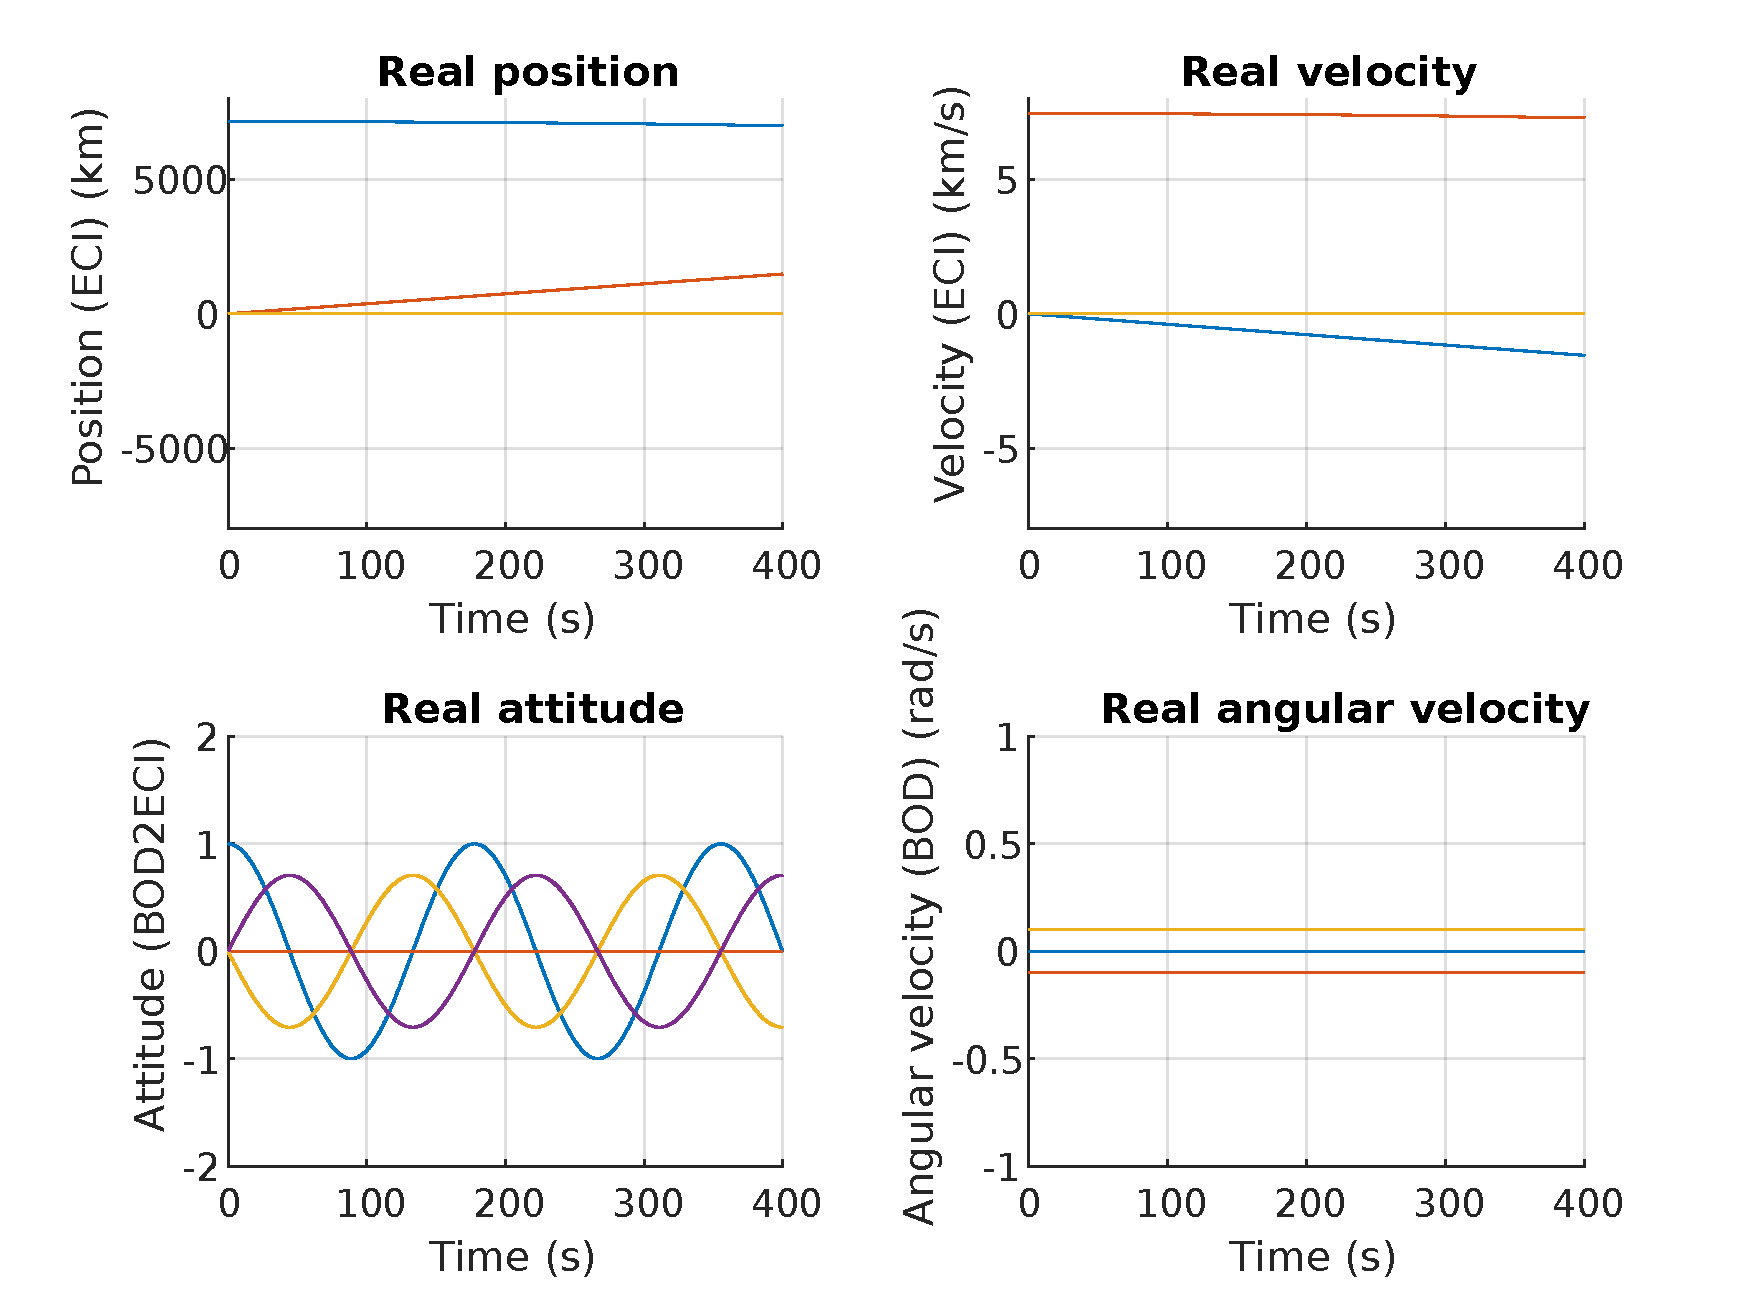
\includegraphics[width=0.8\linewidth]{figures/States.pdf}
    \caption{Your figure caption.}
    \label{fig:3.1}
\end{figure}


\mysection{Rigid Body Mechanics}{Rigid Body Mechanics}
\label{sec:modrigid}

\mysubsection{Kinematics}{Kinematics}
\label{sec:kinematics}

\textcolor{red}{The pose of a rigid body in a refrence frame consists of the position and attitude of the body. The attitude, or orientation of a body-fixed reference frame to a
known reference frame. This is usualy represented by a rotation matrix, often referred to as a direction cosine Matrix (DCM). A rotation about a single coordinate axis
is referred to as a coordinate rotation. A coordinate rotation about the x-,y- and z-axes with angles $\phi$, $\theta$ and $\psi$, of the body can be respectivley
describes as, [Willem de Jong p.23]}

\begin{equation}
    R_x(\phi) = \begin{bmatrix} 
        1 & 0 & 0 \\
        0 & \cos(\phi) & \sin(\phi) \\
        0 & -\sin(\phi) & \cos(\phi)
    \end{bmatrix}
    \label{Eq:3.1}
\end{equation}

\begin{equation}
    R_y(\theta) = \begin{bmatrix} 
        \cos(\phi) & 0 & -\sin(\phi) \\
        0 & 1 & 0 \\
        \sin(\phi) & 0  & \cos(\phi)
    \end{bmatrix}
    \label{Eq:3.2}
\end{equation}

\begin{equation}
    R_z(\psi) = \begin{bmatrix} 
        \cos(\phi) & \sin(\phi) & 0 \\
        -\sin(\phi) & \cos(\phi) & 0 \\
        0 & 0 & 1
    \end{bmatrix}
    \label{Eq:3.3}
\end{equation}

\textcolor{red}{Any rotation in 3D space can be described by three coordinate rotations. The DCM describing the attitude of the target in the camera reference frame
(CRF), $\mathbf{A}_{\mathcal{C}}^{\mathcal{B}}$, can be represented by three Eular angles. Each of the angles corresponds to one coordinate rotation. The order
of the Eular 1-2-3 rotation, shown in Figure 3.5, is expressed as}

\begin{equation}
    \boldsymbol{A}_{\mathcal{C}}^{\mathcal{B}} = R_x(\phi)R_y(\theta)R_z(\psi)
    \label{Eq:3.4}
\end{equation}

\begin{equation}
    \begin{bmatrix}
        a_{1,1} & a_{1,2} & a_{1,3}\\
        a_{2,1} & a_{2,2} & a_{2,3}\\
        a_{3,1} & a_{3,2} & a_{3,3}\\
    \end{bmatrix}
\end{equation}

\begin{equation}
    \begin{bmatrix}
        C\theta C\psi & C\theta S\psi &  -S\theta\\
        S\phi S\theta C\psi - C\phi S\psi & S\phi S\theta S\psi + C\phi C\psi & S\phi C\theta\\
        C\phi S\theta C\psi + S\phi S\psi &  C\phi S\theta S\psi - S\phi C\psi & C\phi C\theta
    \end{bmatrix}
\end{equation}

\textcolor{red}{Where S is the sine function and C is the cosine function. The Eular angles are calculated as follows}

\begin{equation}
    \phi = \arctan2\left(\frac{a_{2,3}}{a_{3,3}}\right)
\end{equation}

\begin{equation}
    \theta = \arctan2\left(\frac{-a_{1,3}}{\sqrt{a_{1,1}^2} + \sqrt{a_{1,2}^2}}\right)
\end{equation}

\begin{equation}
    \psi = \arctan2\left(\frac{a_{1,2}}{a_{1,1}}\right)
\end{equation}

\textcolor{red}{mathematicl singularities occur when using Eular angles to represent large rotations. When both $a_{1,1}$ and $a_{1,2}$ in Equation \ref{Eq:3.4} are zero, the expressions
for $\psi$ and $\theta$ ar undefined. This is known as \textit{gimbal lock}, where the changes in the first and third Eular angles are indistinguishable when the second angle nears
a criticual value. Alternatively, the DCM can be described using quaternions, which do not have these singularities. The quaternion rotation is Figure ?? is expressed by the Eular axis
$\mathbf{\bar{e}}=[e_x,e_y,e_z]^T$ and the angle $\theta$}

\begin{equation}
    \mathbf{q} = \begin{bmatrix} q_s \\ q_x \\ q_y \\ q_z \end{bmatrix}
    = \begin{bmatrix} \cos(\theta/2) \\ e_x\sin(\theta/2) \\ e_y\sin(\theta/2) \\ e_z\sin(\theta/2) \end{bmatrix}
\end{equation}

\begin{figure}[H]
    \centering
    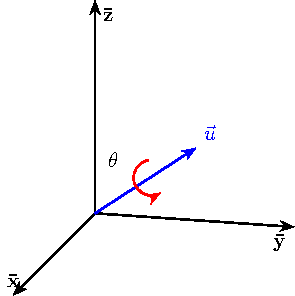
\includegraphics[width=0.3\linewidth]{figures/Quaternion.pdf}
    \caption{Quaternion Rotation}
    \label{fig:3.2}
\end{figure}

\textcolor{red}{The DCM as a function of Quaternion set is expressed as,}

\begin{equation}
    \mathbf{A}_{\mathcal{C}}^{\mathcal{B}} = 
    \begin{bmatrix}
    q_s^2 + q_x^2 - q_y^2 - q_z^2 & 2(q_x q_y - q_s q_z) & 2(q_x q_z + q_s q_y) \\
    2(q_x q_y + q_s q_z) & q_s^2 - q_x^2 + q_y^2 - q_z^2 & 2(q_y q_z - q_s q_x) \\
    2(q_x q_z - q_s q_y) & 2(q_y q_z + q_s q_x) & q_s^2 - q_x^2 - q_y^2 + q_z^2   
    \end{bmatrix}
\end{equation}

\textcolor{red}{Using the normalisation constraint, $q_s^2 + q_x^2 + q_y^2 + q_z^2 = 1$, the DCM Simplifies to,}

\begin{equation}
    \mathbf{A}_{\mathcal{C}}^{\mathcal{B}} = 
    \begin{bmatrix}
    1 - 2(q_y^2 + q_z^2) & 2(q_x q_y - q_s q_z) & 2(q_x q_z + q_s q_y) \\
    2(q_x q_y + q_s q_z) & 1 - 2(q_x^2 + q_z^2) & 2(q_y q_z - q_s q_x) \\
    2(q_x q_z - q_s q_y) & 2(q_y q_z + q_s q_x) & 1 - 2(q_x^2 + q_y^2)   
    \end{bmatrix}
\end{equation}

\textcolor{red}{The body-fixed angular rates of the satellite in CRF, $\mathbf{\omega}_{\mathcal{C}}^{\mathcal{B}}$, is expressed as a function of qauternions by,}

\begin{equation}
    \mathbf{\omega}_{\mathcal{C}}^{\mathcal{B}} = 
    \begin{bmatrix}
        \omega_{bx} \\ \omega_{by} \\ \omega_{bz}
    \end{bmatrix}
    = 2
    \begin{bmatrix}
       -q_x & q_s & -q_z & q_y \\
       -q_3 & q_4 & q_1 & -q_2 \\
       -q_4 & -q_3 & q_2 & q_s 
    \end{bmatrix}
    \begin{bmatrix}
        \dot{q_s} \\ \dot{q_x} \\ \dot{q_y} \\ \dot{q_z}
    \end{bmatrix}
\end{equation}

\textcolor{red}{Inversly the quaternion rates as a function of the body rates are,}

\begin{equation}
    \begin{bmatrix}
        \dot{q_s} \\ \dot{q_x} \\ \dot{q_y} \\ \dot{q_z}
    \end{bmatrix}
    =
    \frac{1}{2}
    \begin{bmatrix}
        0 & -\omega_{bx} & -\omega_{by} & -\omega_{bz}\\
        \omega_{bx} & 0 & \omega_{bz} & -\omega_{by}\\
        \omega_{by} & -\omega_{bz} & 0 & \omega_{bx}\\
        \omega_{bz} & \omega_{by} & -\omega_{bx} & 0 
    \end{bmatrix}
    \begin{bmatrix}
        q_s \\ q_x \\ q_y \\ q_z
    \end{bmatrix}
\end{equation}

\textcolor{red}{Quaternions will be used throughout this thesis for attitude representations. Quaternions do not have ambiguity regarding the order of rotations
and the rotation is around a well-defined axis. The sin and cosine elements of the rotation matrix are already encodedin the quaternion form of the DCM. Therfore,
only one matrix operation is required for attitude transforms, where Eular angles reguire three.}

\mysubsection{Dynamics}{Dynamics}
\label{sec:dynamics}




\mysection{Refrence Frame Transformations}{Refrence Frame Transsformations}

In this masters we are going to encounter a few different refrence frames. To accurateley to create the measurement model we should have an understanding of all the different 
reference models and how to transform from one to another

\subsubsection{Lattitude, longitude and altitude}

The lattitude, longitude of a feature or the position of the satellite is donated with the $\mathcal{L}$. The lattitude of a feature is the position of how high or low it above the
equator, having a range of $-90^{\circ} to 90^{\circ}$. The longitude is based of the greenwich maridian, a longitude line that pases through the north- and south pole, it has a
range of $-180^{\circ} to 180^{\circ}$. The altitude is measured form the the "WGS84" elliptical globe.

\textcolor{blue}{Insert Figure}

\subsection{Earth Ceneterd Earth Fixed}

The Earth Ceneterd Earth Fixed refrence frame is represented by the $\mathcal{F}$ and is very simular to the $\mathcal{L}$ reference frame with the z-axis alligned with the northpole
and the x-axis points at the crossing of the Prime Maridian an the Equator, where the y-axis completes the right hand rule. The x,y and z-axis is defined in kilometers.
To covert from $\mathcal{L}$ to $\mathcal{F}$ is to use a "WGS84" transfomr. Where WGS84 stands for World Geodetic System 1984, which is the standard coordinate system used for
Global Positioning System (GPS). The WGS84 transformation uses a reference ellipsoid that uses a semi-major axis of 6,378 km and a flatting of 1/298.2

\begin{equation}
        \mathbf{A}_{\mathcal{L}}^{\mathcal{F}} = f(WGS84)
\end{equation}

\textcolor{blue}{Insert Figure Here}

\subsection{Earth Ceneterd Inertial}

The Earth Centered Inertial refrence fream (ECI) refrenced by $\mathcal{I}$ shares a refrence frame axis with the ECEF, but is rotated about the z-axis. This rotation is governed
by the rotation speed of the earth $\omega_e$ which is $7.2921\times10^{-5}$ rad/s and time $t$.

\begin{equation}
    \mathbf{A}_{\mathcal{F}}^{\mathcal{I}} = R(\omega_e t) = 
    \begin{bmatrix}
        \cos(\omega_e t) & -\sin(\omega_e t) & 0\\
        \sin(\omega_e t) & \cos(\omega_e t) & 0\\
        0 & 0 & 1
    \end{bmatrix}
\end{equation}

\textcolor{blue}{Insert Figure Here}

\subsection{Orbital reference frame}

The orbital reference frame used is the Local Vertical Local Horizon (LVLH) denoted by $\mathcal{O}$. \textcolor{red}{The LVLH frame is a rotating, orbit-attached corrdinate
system commonly used in spacecraft dynamics. It moves with the satellite and is defined relative to its orbit around Earth}. The x-axis is the "Local Horizon" also called
"along track" pointing forward it is tangent to the orbit and points in the direction of motion. The z-axis is the local vertical and is also called the Nadir direction, it points
to the barycenter of the system, in this case the center of the Earth. The y-axis is called the cross track it completes the right handed system. It points out of the orbital plane,
typically the angular momentum vector direction (normal to the orbit plane).

if $\mathbf{r}$ is the position vector of the satellite and $\mathbf{v}$ is the velocity vector of the satellite.
The equation for the reference frame is:

\begin{align}
    \bar{z}_{\mathcal{O}} &= -\frac{\mathbf{r}}{||\mathbf{r}||} \\
    \bar{y}_{\mathcal{O}} &= \frac{\mathbf{r}\times\mathbf{v}}{||\mathbf{r}\times\mathbf{v}||}\\
    \bar{x}_{\mathcal{O}} &= \bar{y}_{\mathcal{O}}\times\bar{z}_{\mathcal{O}}
\end{align}

For this reference frame there should also be a refrence frame translation introduced. Which is done by substracing $\mathbf{r}$ from the vector

\begin{equation}
    \mathbf{f}_{\mathcal{O}} = \mathbf{A}_{\mathcal{I}}^{\mathcal{O}}\times(\mathbf{f}_{\mathcal{I}} - \mathbf{r}_{\mathcal{I}})
\end{equation}

\textcolor{blue}{Insert Figure Here. This is unfinished explain a bit more. Actually want to change it to the 4x4 transformation matrix}

\subsection{Camera Reference Frame}

The camera refrence frame denoted by $\mathcal{C}$ and the body reference frame $\mathcal{B}$ in this thesis is the same reference frame. This reference frame is transformed
by using your standard quaternion rotaion matrix.

\begin{equation}
    \mathbf{f}_{\mathcal{C}} = \mathbf{A}_{\mathcal{O}}^{\mathcal{C}}\times\mathbf{f}_{\mathcal{O}}
\end{equation}



\mysection{State Estimation}{State Estimation}
\label{sec:modrec}

\mysection{Conclusion}{Conclusion}
\label{sec:modconclusion}
\mychapter{Image Processing}{Image Processing}{}
\label{chap:imgpros}

\mysection{Introduction}{Introduction}
\label{sec:imgintro}

\mysection{Pinhole Camera Model}{Pinhole Camera Model}
\label{sec:imgpinhole}

The ideal pinhole camera can be described as a plane and an optical center (a.k.a) the pinhole. Light will travel from an object throught the optical center.
And hit the plane at the opposite end of the optical center. The distance between the opitical center and the plane is called the focal length $f$.


\begin{figure}[H]
    \centering
    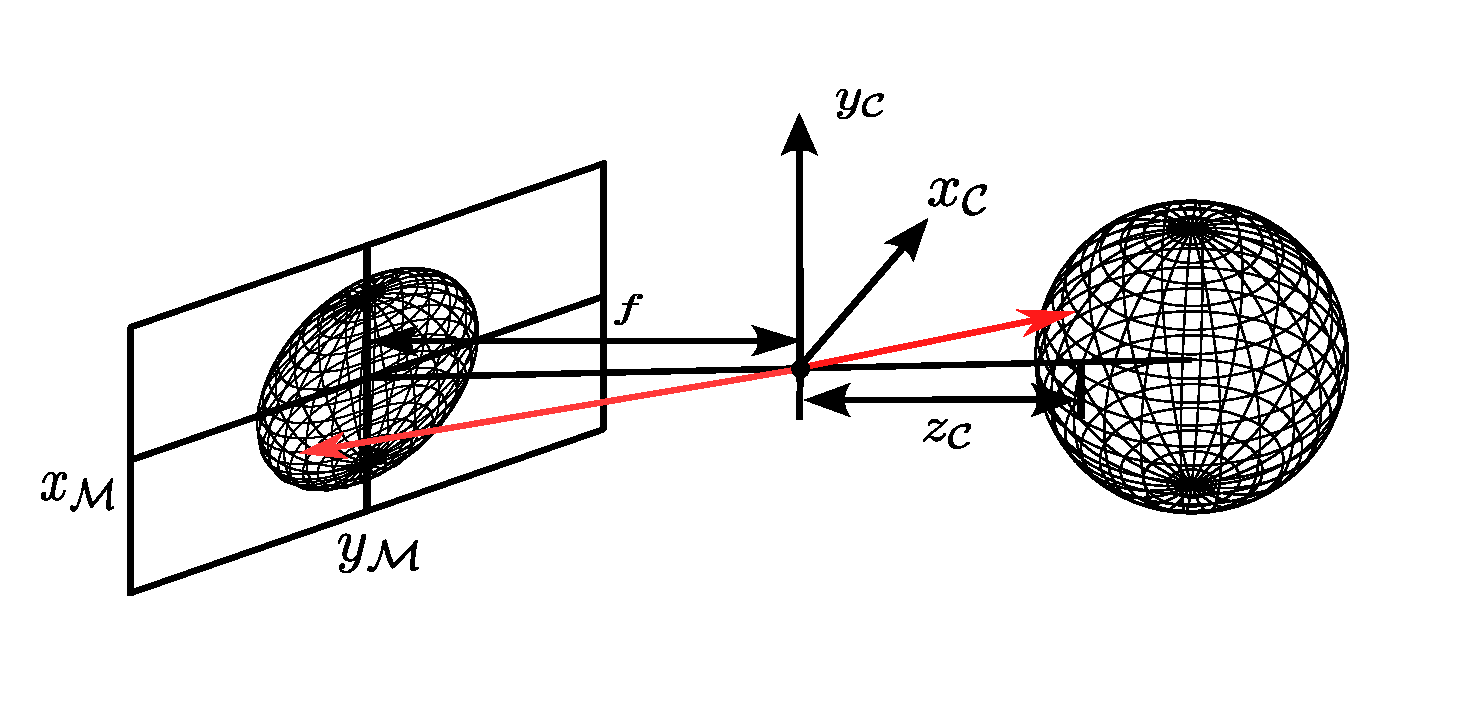
\includegraphics[width=1\linewidth]{figures/imageprocessing/Pinhole.pdf}
    \caption{PinHole Model}
    \label{fig}
\end{figure}


The equation for the pinhole camera model is the following.

\begin{equation}
\begin{bmatrix}
    x_\mathcal{M} \\
    y_\mathcal{M} \\
    1 
\end{bmatrix}
= \frac{-f}{z_\mathcal{C}}
\begin{bmatrix}
    x_\mathcal{C} \\
    y_\mathcal{C} \\
    z_\mathcal{C}
\end{bmatrix}
\end{equation}

As we can see in the figure this also causes the image tp flip.

Also images are measured with the x-axis going from right to left and the y-axis going from top to bottom so one more transformation needs to be done.

\begin{figure}[H]
    \centering
    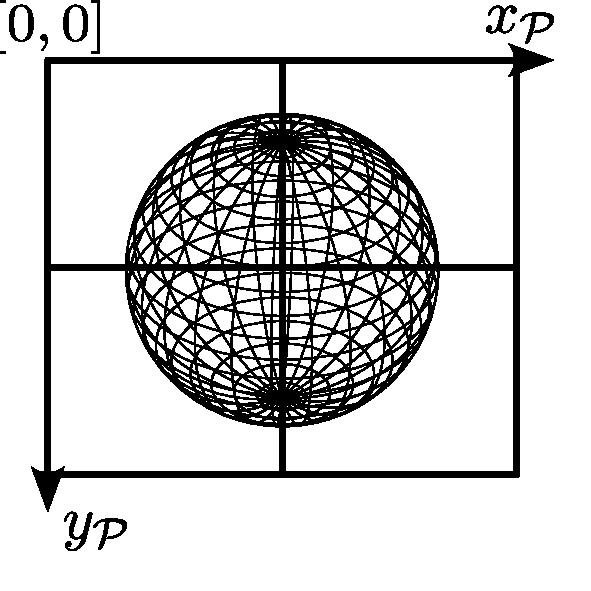
\includegraphics[width=0.5\linewidth]{figures/imageprocessing/ImagePlane.pdf}
    \caption{Image Plane}
    \label{fig4.2}
\end{figure}

\begin{equation}
\begin{bmatrix}
x_\mathcal{P} \\
y_\mathcal{P}
\end{bmatrix}
=
\begin{bmatrix}
    -x_\mathcal{M} + \frac{\text{ImgWidth}}{2} \\
    y_\mathcal{M} + \frac{\text{ImgHeight}}{2}
\end{bmatrix}
\end{equation}


\mysubsection{Intrinsic Camera Parameters}{Intrinsic Camera Parameters}

The projection plane coordinates of the projected point P can be converted into pixel baed measurements by expanding the projection matrix.

A horizontal and verticle scale factor $s_u$ and $s_v$ are defined as 


\begin{equation}
    s_u = \frac{\text{horizontal image resolution}}{\text{horizontal sensor size}}
\end{equation}

\begin{equation}
    s_v = \frac{\text{vertical image resolution}}{\text{vertical sensor size}}
\end{equation}

In the above equations, image resolution refers to the size, in pixels, of the resulting image captures by the modelled camera. Sensor size refers to the physical
size of the sensor, this means the scaling factor can be seen as having a unit of pixels per distance. These scaling factors can be incorporated with the focal length
of the camera to create factors $f_u$ and $f_v$ so that

\begin{equation}
    f_u = s_uf
\end{equation}

\begin{equation}
    f_v =s_vf
\end{equation}

Pixel based coordinates of the projected point $\mathbf{p}$ can be calculated with

\begin{equation}
    s
    \begin{bmatrix}
    u \\
    v \\
    1    
    \end{bmatrix}
    =
    \begin{bmatrix}
        f_u & 0 & 0 \\
        0 & f_v & 0 \\
        0 & 0 & 1
    \end{bmatrix}
    \begin{bmatrix}
        p_x \\ 
        p_y \\
        p_z
    \end{bmatrix}
\end{equation}

Where the s is the scaling factor. The Projection matrix in Equation ... can lastly be expanded with the offsets $o_u$ amd $o_v$ that ensure that the pixel-based
projection plane coordinates are in the lower-right quadrant, as in the convention with digital image. These offsets are defined as

\begin{equation}
    o_u = \frac{\text{horizontal image resolution}}{2}
\end{equation}

\begin{equation}
    o_v = \frac{\text{vertical image resolution}}{2}
\end{equation}

Pixel-based coordinated off the projected point $\mathbf{p}$ can be calculated in the typical convention with

\begin{equation}
    s
    \begin{bmatrix}
        u \\
        v \\
        1
    \end{bmatrix}
    =
    \begin{bmatrix}
    f_u & \alpha & o_u
    0 & f_v & o_v
    0 & 0 & 1
    \end{bmatrix}
    \begin{bmatrix}
        p_x \\
        p_y \\
        p_z
    \end{bmatrix}
\end{equation}

\begin{equation}
    = \mathbf{K}
    \begin{bmatrix}
    p_x \\
    p_y \\
    p_z
    \end{bmatrix}
\end{equation}

where $\mathbf{K}$ is known as the intrinsic matrix a skewing factor of $\alpha$ is added to adjust for skewing affects of the camera.

\mysubsection{Extrensic Camera Paramters}{Extrensic Camera Parameters}

In the equations it is assumed that the point being projected onto the image plane reference is defined in the camera reference frame. This
is not always the case and in certain circumstances the points that have to projected will have to be corrected the camera reference frame first.

An extrinsic camera matrix performs this conversion taks, it is made of a DCM $\mathbf{D}$ and translation vector $\mathbf{t}$ so that 

\begin{equation}
    [\mathbf{D}|\mathbf{t}] =
    \begin{bmatrix}
        d_{11} & d_{12} & d_{13} & t_1 \\
        d_{21} & d_{22} & d_{23} & t_2 \\
        d_{31} & d_{32} & d_{33} & t_3 \\
    \end{bmatrix}
\end{equation}

\begin{equation}
    s
    \begin{bmatrix}
        u \\
        v \\
        1
    \end{bmatrix}
    = \mathbf{K}[\mathbf{D}|\mathbf{t}]
    \begin{bmatrix}
        p_x \\
        p_y \\
        p_z \\
        1
    \end{bmatrix}
\end{equation}

\mysubsection{Back Projection}{Back Projection}

The intrinsic camera matrix discussed is typicall used to project 3D points in the camera referecne frame down to the 2D image plane reference frame. It can
also be used to project 2D coordinates on the image plane reference frame back into 3D space.

Assume the scaling factor $s$ is known or assumed.

The 3D vector can be reconstructed.

\begin{equation}
\mathbf{d} = s*\mathbf{K}^{-1}
\begin{bmatrix}
    u \\
    v \\
    1
\end{bmatrix}
\end{equation}


\mysection{Satellite Image Characteristics}{Satellite Image Characteristics}

\mysubsection{Ground Sample Distance}{Ground Sample Distance}
% Mathematical relationship

Ground Sampling Distance (GSD) is the real-world distance between the centers of two adjacent 
pixels measured on the ground in an image captured by a remote sensing system or satellite. It represents 
the spatial resolution of the imaging sensor and determines the level of detail visible in the image — smaller GSD 
values correspond to higher resolution, allowing finer features on the ground to be distinguished.

Where the mathematical relationship is

\begin{equation}
    GSD = \frac{\text{altitude} * \text{pixelsize} * \text{resolution}}{\text{focal length}}
\end{equation}


% Impact on feature detection accuracy
% Trade oofs with altitude and camera parameters


\mysubsection{Imaging Geometry}{Imaging Geometry}

% Nadir vs off-nadir imaging
% Field of view calculations

The field of view (FOV) of the satellite imager is calculated using the relationship between the camera's focal length, 
sensor dimensions, and pixel size. The vertical field of view is determined by the equation $\text{FOV}_v = 2 \times \arctan\left(\frac{I_y \times p_s}{2f}\right)$, 
where $I_y$ is the image height in pixels, $p_s$ is the pixel size, and $f$ is the focal length. For the horizontal field of view, the image width $I_x$ is 
substituted for $I_y$ in the calculation. This angular field of view defines the observable ground area from the satellite's orbital altitude, with the ground 
sample distance (GSD) providing the metric resolution per pixel according to $\text{GSD} = \frac{p_s \times h}{f}$, where $h$ is the altitude above the target 
surface. These geometric relationships are fundamental to the measurement model, as they establish the transformation between pixel coordinates in the image plane 
and the corresponding angular directions in the camera reference frame, enabling precise feature vector calculations for pose estimation.

% Ground coverage estimation
% Geometric distortions

\mysubsection{Lens Distortions}{Lens Distortions}

% Radial
% Tangential
% Abberations

\mysection{Feature Detection and Description}{Feature Detection and Description}

\mysubsection{Classical Feature Detectors}{Classical Feature Detectors}
% SIFT
\mysubsubsection{SIFT}{SIFT}

Scale-Invariant Feature Transform (SIFT) is a computer vision algorithm designed to detect and describe local features in images that remain 
stable under various transformations including scaling, rotation, and illumination changes. The algorithm operates in four main stages: scale-space extrema 
detection using Difference of Gaussians (DoG), keypoint localization through sub-pixel refinement, orientation assignment based on local gradient histograms, 
and descriptor generation using a 128-dimensional feature vector.

The scale-space representation is constructed by convolving the input image $I(x,y)$ with Gaussian kernels of increasing standard deviation:
\begin{equation}
L(x,y,\sigma) = G(x,y,\sigma) * I(x,y)
\end{equation}
where $G(x,y,\sigma) = \frac{1}{2\pi\sigma^2}e^{-(x^2+y^2)/2\sigma^2}$ is the Gaussian kernel. The DoG function approximates the Laplacian of Gaussian for 
efficient keypoint detection:
\begin{equation}
D(x,y,\sigma) = L(x,y,k\sigma) - L(x,y,\sigma)
\end{equation}
where $k$ is a constant multiplicative factor between adjacent scales.

For each detected keypoint, the dominant orientation is determined by computing the gradient magnitude and direction:
\begin{align}
m(x,y) &= \sqrt{[L(x+1,y) - L(x-1,y)]^2 + [L(x,y+1) - L(x,y-1)]^2} \\
\theta(x,y) &= \arctan\left(\frac{L(x,y+1) - L(x,y-1)}{L(x+1,y) - L(x-1,y)}\right)
\end{align}

The descriptor is constructed by sampling gradients in a 16×16 pixel neighborhood around the keypoint, subdivided into 4×4 blocks with 
8-bin orientation histograms, resulting in a 128-dimensional feature vector ($4 \times 4 \times 8 = 128$). Each descriptor element is weighted by 
the gradient magnitude and a Gaussian window centered at the keypoint. The resulting 128-dimensional descriptor provides robust matching capabilities 
across different viewing conditions, making SIFT particularly suitable for satellite imagery where features must be reliably detected despite changes in lighting, 
seasonal variations, and slight geometric distortions. However, the computational complexity of SIFT can be limiting for real-time applications, requiring careful 
consideration of the trade-off between feature quality and processing speed in resource-constrained satellite systems.

% SURF
\mysubsubsection{SURF}{SURF}

Speeded-Up Robust Features (SURF) is a computer vision algorithm developed as a faster alternative to SIFT while maintaining comparable performance 
in feature detection and description. SURF achieves computational efficiency through the use of integral images and approximations of the Laplacian of 
Gaussian operator, making it particularly suitable for real-time applications in resource-constrained satellite systems.

The algorithm utilizes integral images $I_{\Sigma}(x,y)$ to enable rapid computation of rectangular area sums:
\begin{equation}
I_{\Sigma}(x,y) = \sum_{i=0}^{i \leq x} \sum_{j=0}^{j \leq y} I(i,j)
\end{equation}
where $I(i,j)$ represents the intensity at pixel $(i,j)$. This allows any rectangular sum to be computed in constant time using only four array references.

SURF approximates the Laplacian of Gaussian using box filters that can be evaluated efficiently with integral images. The determinant of the Hessian matrix is used for keypoint detection:
\begin{equation}
\text{Det}(\mathbf{H}) = D_{xx}D_{yy} - (0.9D_{xy})^2
\end{equation}
where $D_{xx}$, $D_{yy}$, and $D_{xy}$ are the convolution responses of the image with the second-order Gaussian derivatives, approximated using box filters. The factor 0.9 is an empirical weight to balance the expression.

For orientation assignment, SURF computes Haar wavelet responses in the $x$ and $y$ directions within a circular neighborhood:
\begin{align}
d_x &= \text{Haar}_x * I(x,y) \\
d_y &= \text{Haar}_y * I(x,y)
\end{align}
The dominant orientation is determined by summing all responses within a sliding window of $\frac{\pi}{3}$ radians.

The SURF descriptor is typically 64-dimensional (compared to SIFT's 128), constructed by dividing a 20×20 pixel region around the keypoint into 4×4 sub-regions. 
For each sub-region, the wavelet responses are summed to create a 4-dimensional descriptor vector $\mathbf{v} = [\sum d_x, \sum d_y, \sum |d_x|, \sum |d_y|]$. 
This results in a $4 \times 4 \times 4 = 64$-dimensional descriptor that provides robust matching while requiring significantly less computational resources 
than SIFT, making it advantageous for satellite pose estimation applications where processing efficiency is critical.

% ORB
\mysubsubsection{ORB}{ORB}

Oriented FAST and Rotated BRIEF (ORB) is a binary feature descriptor that combines the FAST keypoint detector with the BRIEF descriptor, 
enhanced with orientation compensation to achieve rotation invariance. ORB is designed for real-time applications and provides significant computational 
advantages over SIFT and SURF, making it particularly suitable for resource-constrained satellite systems where processing efficiency is paramount.

The FAST (Features from Accelerated Segment Test) detector identifies keypoints by examining the intensity values of 16 pixels arranged in a circle around 
a candidate point $p$. A pixel $p$ is classified as a corner if there exists a set of $n$ contiguous pixels in the circle that are all brighter than $I_p + t$ or 
all darker than $I_p - t$, where $I_p$ is the intensity of pixel $p$ and $t$ is a threshold:
\begin{equation}
\text{FAST}(p) = \begin{cases}
1 & \text{if } \exists \text{ arc of length } n \text{ such that } \forall x \in \text{arc}: |I_x - I_p| > t \\
0 & \text{otherwise}
\end{cases}
\end{equation}

To achieve rotation invariance, ORB computes the intensity centroid to determine keypoint orientation. The moments of a patch are calculated as:
\begin{align}
m_{pq} &= \sum_{x,y} x^p y^q I(x,y) \\
\text{Centroid: } \mathbf{C} &= \left(\frac{m_{10}}{m_{00}}, \frac{m_{01}}{m_{00}}\right)
\end{align}
The orientation angle is then determined by:
\begin{equation}
\theta = \arctan\left(\frac{m_{01}}{m_{10}}\right)
\end{equation}

The BRIEF descriptor is modified to create rBRIEF (rotated BRIEF) by applying a rotation matrix to the sampling pattern. For a set of $n$ binary tests, 
each test $\tau$ compares the intensities of two pixels:
\begin{equation}
\tau(p; x, y) = \begin{cases}
1 & \text{if } p(x) < p(y) \\
0 & \text{otherwise}
\end{cases}
\end{equation}
The rotated sampling pattern is computed as:
\begin{equation}
\mathbf{S}_{\theta} = \mathbf{R}_{\theta} \mathbf{S}
\end{equation}
where $\mathbf{R}_{\theta}$ is the rotation matrix and $\mathbf{S}$ is the original sampling pattern.

The final ORB descriptor is a 256-bit binary string computed by applying the rotated BRIEF tests. This binary representation 
enables extremely fast matching using the Hamming distance, computed as:
\begin{equation}
d_H(\mathbf{a}, \mathbf{b}) = \sum_{i=1}^{n} a_i \oplus b_i
\end{equation}
where $\oplus$ denotes the XOR operation. The computational efficiency and low memory requirements of ORB make it ideal for satellite 
pose estimation applications where real-time performance and limited computational resources are critical constraints.


\mysubsubsection{Comparison}{Comparison}

% \mysubsection{Feature Description}{Feature Description}
% \label{sec:featuredescription}

% Local feature descriptors play a crucial role in satellite pose estimation by providing robust representations of image features 
% that can be matched across different viewing conditions. These descriptors encode the local appearance of image regions around detected 
% keypoints, creating distinctive signatures that enable reliable correspondence matching between images captured at different times, orientations, and lighting conditions.

% \mysubsubsection{Invariance Properties}{Invariance Properties}
% \label{sec:invarianceproperties}

% The effectiveness of feature descriptors in satellite applications depends critically on their invariance properties. Scale invariance ensures 
% that features remain detectable as the satellite altitude changes or when using different zoom levels. This is particularly important for Earth 
% observation satellites that may operate at varying altitudes or employ different imaging modes. Rotation invariance is essential for satellites 
% that experience attitude changes, as the same ground features must be recognizable regardless of the satellite's orientation relative to the Earth's surface.

% Illumination invariance addresses the challenge of varying lighting conditions caused by solar angle changes, seasonal variations, and atmospheric 
% effects. For satellite imagery, this property is vital as the same geographic features may be observed under drastically different illumination conditions 
% throughout the orbital period. Affine invariance provides robustness against perspective distortions that occur when observing the same ground features from 
% slightly different viewpoints, which is common in satellite imaging due to orbital mechanics and attitude variations.

% \mysubsubsection{Descriptor Matching Strategies}{Descriptor Matching Strategies}
% \label{sec:descriptormatching}

% Feature matching in satellite pose estimation typically employs distance-based similarity measures to establish correspondences between descriptors. 
% For floating-point descriptors like SIFT and SURF, the Euclidean distance provides a natural similarity metric:
% \begin{equation}
% d_E(\mathbf{f}_1, \mathbf{f}_2) = \sqrt{\sum_{i=1}^{n} (f_{1i} - f_{2i})^2}
% \end{equation}
% where $\mathbf{f}_1$ and $\mathbf{f}_2$ are $n$-dimensional descriptor vectors.

% For binary descriptors like ORB, the Hamming distance offers computational efficiency:
% \begin{equation}
% d_H(\mathbf{b}_1, \mathbf{b}_2) = \sum_{i=1}^{n} b_{1i} \oplus b_{2i}
% \end{equation}
% where $\oplus$ represents the XOR operation.

% The nearest neighbor matching strategy identifies the closest descriptor in the database, while the ratio test introduced by Lowe provides 
% additional robustness by comparing the distances to the first and second nearest neighbors:
% \begin{equation}
% \text{Ratio test: } \frac{d_1}{d_2} < \tau
% \end{equation}
% where $d_1$ and $d_2$ are the distances to the first and second nearest neighbors, respectively, and $\tau$ is a threshold typically set to 0.8.

% \mysubsubsection{Robustness to Viewpoint Changes}{Robustness to Viewpoint Changes}
% \label{sec:viewpointrobustness}

% Satellite pose estimation requires descriptors that maintain distinctiveness across moderate viewpoint changes. The challenge arises from the 
% fact that satellites observe the Earth from different positions along their orbital path, creating subtle but significant changes in the appearance 
% of ground features. Viewpoint invariance is typically achieved through normalization techniques that account for local geometric transformations.

% SIFT addresses viewpoint changes through its multi-scale pyramid representation and gradient-based orientation assignment, which provides robustness 
% to viewpoint variations up to approximately 30 degrees. SURF employs similar strategies but with computational optimizations, while ORB relies on the 
% intensity centroid method for orientation normalization.

% For satellite applications, additional robustness can be achieved through descriptor pooling techniques, where multiple descriptors from the same feature 
% are combined to create a more stable representation. Geometric verification using methods such as RANSAC (Random Sample Consensus) helps eliminate false matches 
% that may arise from descriptor ambiguities:
% \begin{equation}
% \mathbf{H} = \arg\min_{\mathbf{H}} \sum_{i=1}^{n} \rho(||\mathbf{p}_i' - \mathbf{H}\mathbf{p}_i||)
% \end{equation}
% where $\mathbf{H}$ is the homography matrix, $\mathbf{p}_i$ and $\mathbf{p}_i'$ are corresponding points, and $\rho$ is a robust cost function.

% The combination of invariant descriptors and robust matching strategies forms the foundation for reliable feature tracking in satellite pose estimation 
% systems, enabling accurate determination of spacecraft position and attitude through visual odometry and simultaneous localization and mapping (SLAM) techniques.

% \mysubsection{Feature Quality Assessment}{Feature Quality Assessment}


\mysection{Measurement Extraction}{Measurement Extraction}
\label{sec:imgmesurement}

\mysubsection{Image Generation}{Image Generation}

\mysubsubsection{Rendering the Earth}{Rendering the Earth}

To create an image

Fisrt a High resolution image is sticth in QGIS, a type fo Geographic information system, used to open an edit geolocated images.
Images a downloaded from the copernicus with a GSD of 15 m.

\textcolor{blue}{Insert Image of Paris}
\textcolor{blue}{Inert Image of Pyramids}
\textcolor{blue}{Insert Image of Hawaii Volcano}

After an high resolution image is sitched. It is rasterised.
This rasterised image with all its goelocation data is then projected onto a WGS84 ellipsoid.

\begin{figure}[H]
    \centering
    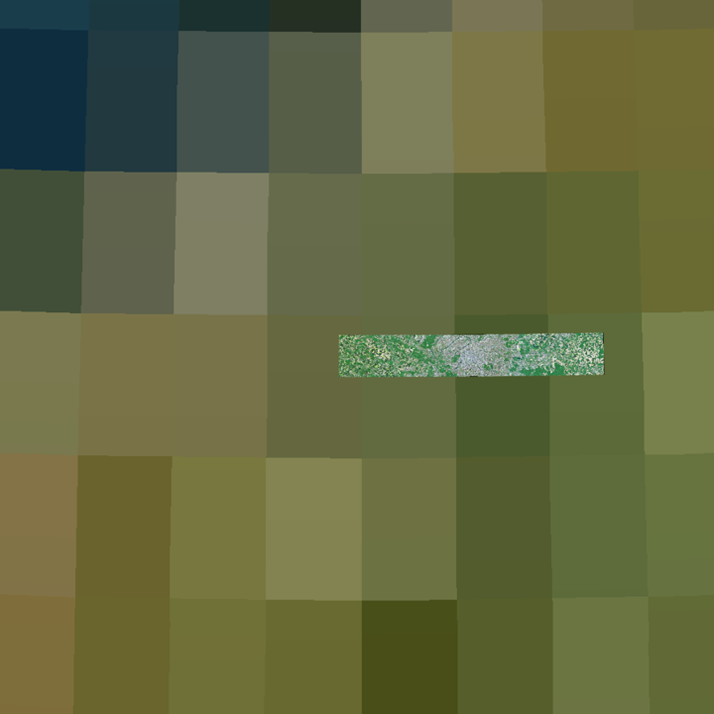
\includegraphics[width=0.5\linewidth]{figures/imageprocessing/HighResImage.png}
    \caption{High Resolution Image projected on Ellipsoid}
    \label{}
\end{figure}

The Low resolution Earth in the Backgorund is used as a place holder to test results

\mysubsection{Earth Tracker Algorithm}{Earth Tracker Algorithm}

The Earth Tracker works on the same principle as Back projection.

\textbf{Step 1: Translate pixels to optical center}

The second step involes translating the pixel cooridnates to the optical center as the origin. This transformation accounts for the camera's principle point
offset, where $I_x$ and $I_y$ represent width and height, repsectivly. The resulting coordinate vector $\mathbf{f}_{\mathcal{M/S}}$ represents position Relative
to the camera boresight.

\begin{equation}
    \mathbf{f}_{\mathbf{M/S}} = 
    \begin{bmatrix}
        f_\mathcal{M} - \frac{I_x}{2} \\
        f_\mathcal{M} - \frac{I_y}{2}
    \end{bmatrix}
    \text{(Pixels)}
\end{equation}

\begin{figure}[H]
    \centering
    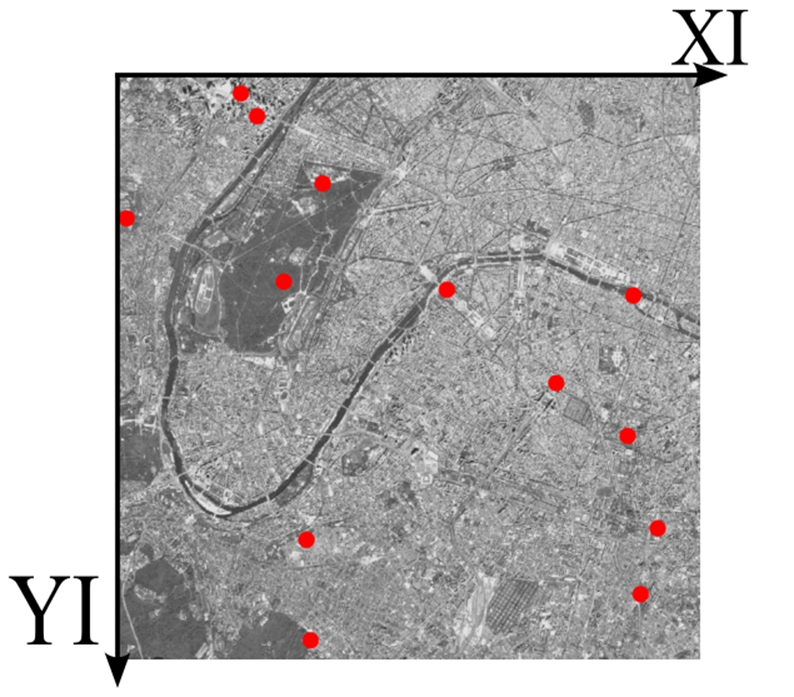
\includegraphics[width=0.5\linewidth]{figures/imageprocessing/IMG1.png}
    \caption{Origin Correction}
    \label{}
\end{figure}

\begin{figure}[H]
    \centering
    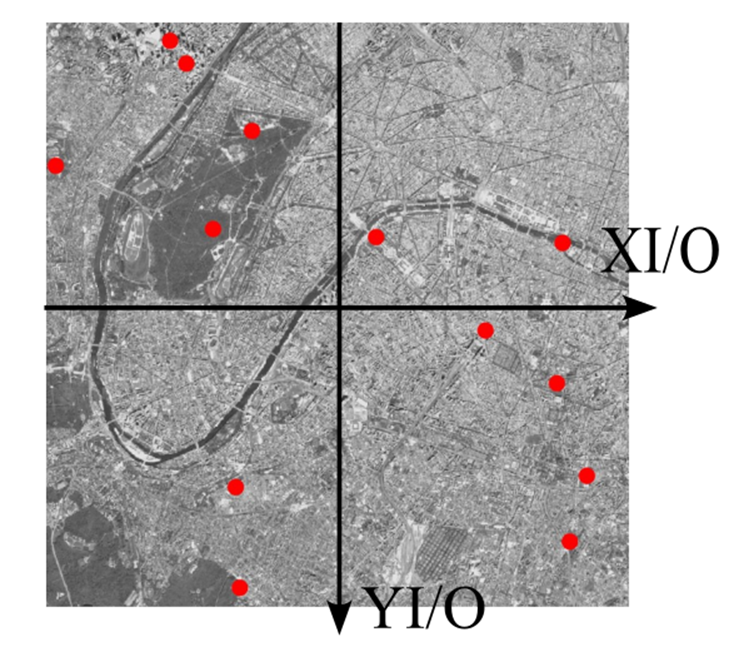
\includegraphics[width=0.5\linewidth]{figures/imageprocessing/IMG2.png}
    \caption{Origin Correction 2}
    \label{}
\end{figure}

\textbf{Step 2: Three-Dimentional Ray Vector Construction}

This step transform the 2 dimensional pixel coordinates into the three-dimensional direction vector in the camera frame. The vector $\mathbf{f}_\mathcal{M/F}$ represents
the feqture direction relative to the camera focal point, where the z-component is dtermined by the effective focal lenght in pixels

\begin{equation}
    \mathbf{f}_\mathcal{M/F} = 
    \begin{bmatrix}
        f_{\mathcal{M/S_x}} \\
        f_{\mathcal{M/S_y}} \\
        \frac{fl}{ps}
    \end{bmatrix}
\end{equation}

\textbf{Step 3: Scale dorection vector}

The 3rd step performs a cordinate transformation to orient the feature vector in the appropriate referecne direction. This operation inverts and scales the vector so that it
is correct in the camera reference frame

The sacling used is the assumed GSD

\begin{equation}
    \mathbf{f} = GSD \times \mathbf{f}
\end{equation}

\mysubsection{Geolocation Process}{Geolocation Process}

For the geolocation.

\textbf{Step 1: Chip Image}

\textbf{Step 2: Chip features}

\textbf{Step 3: Use SIFT for feauture matching}

\textbf{Step 4: Add geolocation}



\mychapter{State Estimation}{State Estimation}{}
\label{chap:stateestimation}

\mysection{Introduction}{Introduction}
\label{sec:stateintro}

\mysection{Recursive Estimation}{Recursive Estimation}
\label{sec:stateEKF}

This section describes the element of recrusive estimators along with a few commonly-used estimators in the fields of localisation and tracking. A recursive estimoter uses the previous
distrubution over a set of systm states and curent sensor data to estimte the current state distribution. Figure 3.1 illustrates the basic workings of a discrete recursive filter.

\begin{figure}[H]
    \centering
    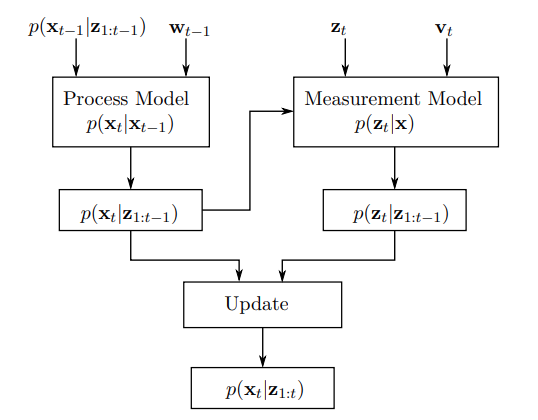
\includegraphics[width=0.5\linewidth]{figures/StateEstimation/Recursive Estimation.png}
    \caption{Recursive estimator algorithm flowchart}
    \label{}
\end{figure}

The state vector is represented by $\mathbf{x}_t$ for the estimation problem in the discrete time domain. The process, or the state transition function, is expressed As
\begin{equation}
    \mathbf{x}_t = \mathbf{f}(\mathbf{x}_{t-1},\mathbf{u}_{t-1},\mathbf{w}_{t-1})
\end{equation}

where $\mathbf{f}$ is either a linear or non-linear transtion fucntion and $\mathbf{w}_t$ represents the process noise. New observation data, $\mathbf{z}_t$, is available at
discrete timesteps and can be related to $\mathbf{x}_t$ by the measurement function,

\begin{equation}
    \mathbf{z}_t = \mathbf{h}(\mathbf{x}_t,\mathbf{v}_t)
\end{equation}

The measurement uncertainty is represented by $\mathbf{v}_t$ and $\mathbf{h}$ is the observation model, which can also either be linear or non-linear. The goal is to obtain the
posterior distribution, $p(\mathbf{x}|\mathbf{z}_{1:t})$, over the state vector $\mathbf{x}_t$. This is done by recursively performing the process and measurement updates.

At a time $t$, the posterior distribution over $\mathbf{x}_{t-1}$ at time $t-1$ is known and the prior distribution at t is calcualted As

\begin{equation}
    p(\mathbf{x}_t|\mathbf{z}_{1:t-1}) = \int p(\mathbf{x}_t|\mathbf{x}_{t-1})p(\mathbf{x}_{t-1}|\mathbf{z}_{1:t-1})\ d\mathbf{x}_{t-1}
\end{equation}

The measruement update is used to calculate the new posterior, at time $t$ , given the prior state distribution according to Bayes' rule,

\begin{equation}
    p(\mathbf{x}_t|\mathbf{z}_{1:t}) = 
    \frac{p(\mathbf{z}_t|\mathbf{x}_t)p(\mathbf{x}_t|\mathbf{z}_{1:t-1})}{p(\mathbf{z}_t|\mathbf{z}_{1:t-1})}
\end{equation}

The Kalman filter is a popular estimator used in pose estimation porblems. It is a special case of the Bayes filter, where the Guassian noise distributions are assumed.
The assumption is also made that the initial distibution of the system can be represented by a Gaussian distribution. A control and measurement update is executed
at each sampling instant to update the distibutionover the states. If the previous state distribution is Gaussian, then the updated current distribution will also be Gaussian
and therefore the best estimate is chosen as the mean of the distribution.

Differen variants of the Kalman Filter exists, of which the extended and unscented Kalman Filter are the most popular, eah with their own unique characteristics.

The extended Kalman Filter (EKF) overcomes the restrictions of the linear filter by approximating non-linear functions to be linear using a first-order Taylor expansion.
The mean position of the state vector is used as the linearisation point around which the tangent of the non-linear function is calcualted, allowing the use of standard
Kalman Filter equations. It is typically more efficient than other non-linear filters which sometimes comes at a cost or reduced accuracy.

The unscented Kalman Filter (UKF) uses stochiatic linearisation to deal with non-linear systems. Given a distribution with a known mean and covariance, a set of weighted points,
known as sigma points, are chosen and transformed using the non-linear function. A new distribution is determined from the transformed sigma points. The process and observation
functions do not need to be differentiable and the output is based on vlaues in a larger region, rather than a local approximation.

\mysection{Kalman Filter}{Kalman Filter}


Kalman filters are well suited for localistation problems since the nature of these systems are normally non-linear. Both the linear and non-linear variants of the Kalman Filter
are concenerd with estimating states using motion model to perform this data fusion. The following equations are used to model the system.

\begin{equation}
    \mathbf{x}_t = A_t\mathbf{x}_{t-1} + B\mathbf{u}_{t-1} + \mathbf{\epsilon}
    \mathbf{z}_t = C_t\mathbf{x}_t + \mathbf{\zeta}
\end{equation}

where

\begin{equation}
    \epsilon = \mathcal{N}(\mathbf{0};R)
    \zeta = \mathcal{N}(\mathbf{0};Q)
\end{equation}

The matrices R and Q are the known covarianve matrices of the process and observation noise, repsectivly and the matrices A, B and C form part of the linear functions.

These equations can be used to calculate the posterior distrobution

\begin{equation}
    p(\mathbf{y}_t|\mathbf{u}_{1:t},\mathbf{z}_{1:t}) = \mathcal{N}(\mu_t ;\Sigma_t)
\end{equation}

The state estimation problem in this project makes use of non-linear system models, and a high-dimensinal state space. The EKF is well suited for this problem, since it
accomodates non-linear process and observation models and is capable of dealing with high-dimensional state spaces. The EKF os often use for the SLAM problem and is well
known in the field of robotics and localisation.

The rigid body motion models and measurements models of systems are, however, non-linear. Therefore, a general non-linear description is used for the motion and measurement models

\begin{equation}
    \mathbf{y}_t = \mathbf{g}(\mathbf{y}_{t-1},\mathbf{u}_t) + \boldsymbol{\epsilon}
\end{equation}

\begin{equation}
    \mathbf{z}_t = \mathbf{h}(\mathbf{y}_t) + \boldsymbol{\zeta}     
\end{equation}

The motion and measurement functions, $\mathbf{g}$ and $\mathbf{h}$, are non-linear vector functions.  These are linearised to enable the use of the Kalman filter equations. 
The non-linear vector functions, $\mathbf{f}(\mathbf{x}) = [f_1(\mathbf{x}),f_2(\mathbf{x}),...,f_m(\mathbf{x})]^T$, is linearised around its mean value, $\mu$, using
a Taylor series expansion.

\begin{equation}
    \mathbf{f}(\mathbf{x}) \approx \mathbf{f}(\boldsymbol{\mu}) + \mathbf{f}'(\boldsymbol{\mu})(\mathbf{x}-\boldsymbol{\mu})
\end{equation}

where


\begin{equation}
  \begin{aligned}
    \mathbf{f}'(\mathbf{x})
      &= \mathit{F}(\mathbf{x})
       = \frac{\partial \mathbf{f}(\mathbf{x})}{\partial \mathbf{x}} \\
      &=
    \begin{bmatrix}
      \dfrac{\partial f_1}{\partial x_1} & \cdots & \dfrac{\partial f_1}{\partial x_n} \\
      \vdots & \ddots & \vdots \\
      \dfrac{\partial f_m}{\partial x_1} & \cdots & \dfrac{\partial f_m}{\partial x_n}
    \end{bmatrix}_{m \times n}
  \end{aligned}
\end{equation}

$\mathit{F}(\mathbf{x})$ is referred to as the Jacobian matrix. Using this linearisation, the vector function, $\mathbf{g}$ and $\mathbf{h}$
are approximated as,

\begin{equation}
    \mathbf{y}_{t-1}, \mathbf{u}_t \approx \mathbf{g}(\boldsymbol{\mu}_{t-1}, \mathbf{u}_t) + \mathbf{G}_t (\mathbf{y}_{t-1} - \boldsymbol{\mu}_{t-1})
\end{equation}

\begin{equation}
    \mathbf{h}(\mathbf{y}_t) \approx \mathbf{h}(\boldsymbol{\mu}_t) + \mathbf{H}_t (\mathbf{y}_t - \boldsymbol{\mu}_t)
\end{equation}

where \( \mathbf{G}_t \) and \( \mathbf{H}_t \) are the Jacobian matrices of \( \mathbf{g} \) and \( \mathbf{h} \), respectively. This linearisation leads to the approximate distribution

\begin{equation}
    p(\mathbf{y}_t \mid \mathbf{u}_{1:t}, \mathbf{z}_{1:t}) \approx \mathcal{N}(\boldsymbol{\mu}_{t \mid t}, \boldsymbol{\Sigma}_{t \mid t})
\end{equation}



\mysection{System Modelling}{System Modelling}
\label{sec:statesystemmodel}

\begin{figure}[htbp]
    \centering
    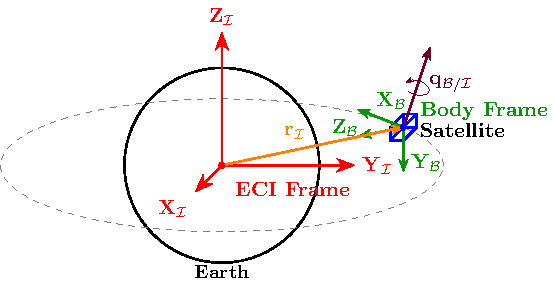
\includegraphics[width=0.8\textwidth]{figures/Figure1.pdf}
    \caption{Satellite pose estimation concept showing orbital geometry, reference frames}
    \label{fig:System Modelling}
\end{figure}

As we can see in Figure \ref{fig:System Modelling} to determine the pose of the satellite the position and the attitude of the satellite in the ECI reference frames needs to be
determines

\begin{equation}
    \mathbf{x}_t =
    \begin{bmatrix}
        \mathbf{r}_\mathcal{I} & \mathbf{v}_\mathcal{I} & \mathbf{q}_\mathcal{B/I} & \boldsymbol{\omega}_\mathcal{B/I}^\mathcal{B}
    \end{bmatrix}
    ^T
\end{equation}

\mysubsection{Motion Model}{Motion Model}
\label{sec:statemotionmodel}

The rotation of the satellite body is non-linear and the satellite motion from one timestep to the next when using Newton-Eular coupling can be described by the vector function
$\mathbf{g}$,

\begin{equation}
    \mathbf{x}_t = \mathbf{g}(\mathbf{x}_{t-1},\mathbf{u}_t) + \boldsymbol{\epsilon}
\end{equation}

which is expanded to,

\begin{equation}
    \mathbf{x}_t
    =
    \begin{bmatrix}
        r_{x,t} \\
        r_{y,t} \\
        r_{z,t} \\
        v_{x,t} \\
        v_{y,t} \\
        v_{z,t} \\
        q_{s,t} \\
        q_{x,t} \\
        q_{y,t} \\
        q_{z,t} \\
        \omega_{x,t} \\
        \omega_{y,t} \\
        \omega_{z,t} \\
    \end{bmatrix}
    = \mathbf{x}_{t-1} +
    \begin{bmatrix}
        v_{x,t-1} \\
        v_{x,t-1} \\
        v_{x,t-1} \\
        -\frac{\mu}{|\mathbf{r}|^3}*r_{x,t-1} + J2_{x,t-1} \\
        -\frac{\mu}{|\mathbf{r}|^3}*r_{y,t-1} + J2_{y,t-1} \\
        -\frac{\mu}{|\mathbf{r}|^3}*r_{z,t-1} + J2_{z,t-1} \\
        \frac{1}{2}(-\omega_{x,t-1}q_{x,t-1} - \omega_{y,t-1}q_{y,t-1} - \omega_{z,t-1}q_{z,t-1}) \\
        \frac{1}{2}( \omega_{x,t-1}q_{s,t-1} + \omega_{z,t-1}q_{y,t-1} - \omega_{y,t-1}q_{z,t-1}) \\
        \frac{1}{2}( \omega_{y,t-1}q_{s,t-1} - \omega_{z,t-1}q_{x,t-1} + \omega_{x,t-1}q_{z,t-1}) \\
        \frac{1}{2}( \omega_{z,t-1}q_{s,t-1} + \omega_{y,t-1}q_{x,t-1} - \omega_{x,t-1}q_{y,t-1}) \\
        \frac{1}{\mathit{I}_{xx}}(\mathit{I}_{yy}-\mathit{I}_{zz})\omega_{y,t-1}\omega_{z,t-1} \\
        \frac{1}{\mathit{I}_{yy}}(\mathit{I}_{zz}-\mathit{I}_{xx})\omega_{z,t-1}\omega_{x,t-1} \\
        \frac{1}{\mathit{I}_{zz}}(\mathit{I}_{xx}-\mathit{I}_{yy})\omega_{x,t-1}\omega_{y,t-1}
    \end{bmatrix}
    \Delta t + 
    \begin{bmatrix}
        0 \\
        0 \\
        0 \\
        0 \\
        0 \\
        0 \\
        0 \\
        0 \\
        0 \\
        0 \\
        \mathit{T}_x/\mathit{I}_x \\
        \mathit{T}_y/\mathit{I}_y \\
        \mathit{T}_z/\mathit{I}_z
    \end{bmatrix}
\end{equation}

The body-fixed axes of the target are chosen to coincide with its principle axes of inertia. The principle moment of inertia are given barycenter

\begin{equation}
    \mathbf{I}_\mathcal{B} = 
    \begin{bmatrix}
        \mathit{I}_{xx} & 0 & 0 \\
        0 & \mathit{I}_{yy} & 0 \\
        0 & 0 & \mathit{I}_{zz}
    \end{bmatrix}
\end{equation}

External torques, $\mathit{T}_x$, $\mathit{T}_y$ and $\mathit{T}_z$, are asssumed to be zero and there is thus no control input, $\mathbf{u}_t$. 

Thus 

\begin{equation}
    \mathbf{x}_t = \mathbf{g}(\mathbf{x}_{t-1})
\end{equation}

where

\begin{equation}
    \mathbf{x}_t
    =
    \begin{bmatrix}
        r_{x,t} \\
        r_{y,t} \\
        r_{z,t} \\
        v_{x,t} \\
        v_{y,t} \\
        v_{z,t} \\
        q_{s,t} \\
        q_{x,t} \\
        q_{y,t} \\
        q_{z,t} \\
        \omega_{x,t} \\
        \omega_{y,t} \\
        \omega_{z,t} \\
    \end{bmatrix}
    = \mathbf{x}_{t-1} +
    \begin{bmatrix}
        v_{x,t-1} \\
        v_{x,t-1} \\
        v_{x,t-1} \\
        -\frac{\mu}{|\mathbf{r}|^3}*r_{x,t-1} + J2_{x,t-1} \\
        -\frac{\mu}{|\mathbf{r}|^3}*r_{y,t-1} + J2_{y,t-1} \\
        -\frac{\mu}{|\mathbf{r}|^3}*r_{z,t-1} + J2_{z,t-1} \\
        \frac{1}{2}(-\omega_{x,t-1}q_{x,t-1} - \omega_{y,t-1}q_{y,t-1} - \omega_{z,t-1}q_{z,t-1}) \\
        \frac{1}{2}( \omega_{x,t-1}q_{s,t-1} + \omega_{z,t-1}q_{y,t-1} - \omega_{y,t-1}q_{z,t-1}) \\
        \frac{1}{2}( \omega_{y,t-1}q_{s,t-1} - \omega_{z,t-1}q_{x,t-1} + \omega_{x,t-1}q_{z,t-1}) \\
        \frac{1}{2}( \omega_{z,t-1}q_{s,t-1} + \omega_{y,t-1}q_{x,t-1} - \omega_{x,t-1}q_{y,t-1}) \\
        \frac{1}{\mathit{I}_{xx}}(\mathit{I}_{yy}-\mathit{I}_{zz})\omega_{y,t-1}\omega_{z,t-1} \\
        \frac{1}{\mathit{I}_{yy}}(\mathit{I}_{zz}-\mathit{I}_{xx})\omega_{z,t-1}\omega_{x,t-1} \\
        \frac{1}{\mathit{I}_{zz}}(\mathit{I}_{xx}-\mathit{I}_{yy})\omega_{x,t-1}\omega_{y,t-1}
    \end{bmatrix}
    \Delta t
\end{equation}

\mysubsection{Measurement Model}{Measurement Model}
\label{sec:statemeasuremtmodel}

\mysubsection{Earth Tracker Measurement Model}{Earth Tracker Measurement Model}

The Earth Tracker sends 2 inputs to the EKF, the measurement of the Earth tracker itself 

\begin{equation}
    \mathbf{z}_{ET} = \mathbf{f}_\mathcal{B} =
    \begin{bmatrix}
        x_\mathcal{B} \\
        y_\mathcal{B} \\
        z_\mathcal{B}
    \end{bmatrix}
\end{equation}

And the Geolocated feature vector through feature mathcing also refered to as the catalogue vector. $ \mathbf{f}_\mathcal{R}$

To transform this vector into a vector to be comparable to the measurement.

\begin{equation}
    \mathbf{f}_\mathcal{B} = \mathbf{A}_{\mathcal{I},t}^\mathcal{B} \times \mathbf{A}_{\mathcal{R},t}^\mathcal{I} \times \mathbf{f}_\mathcal{R}
\end{equation}


Where $\mathbf{A}_{\mathcal{O},t}^\mathcal{B}$ is a function of the the quaternion $\mathbf{q}_\mathcal{B/I}$





\mysubsection{Other Sensor Measurment model}{Other Sensor Measruement Models}

\textbf{GPS}

For the GPS it measures position in the ECEF reference frame, so it need to be converted to toe ECI reference frame.

\begin{equation}
    \mathbf{H}_{GPS} = 
    \begin{bmatrix}
        \cos(\omega_et) & -\sin(\omega_et) & 0 & \mathbf{0}_{1\times10} \\
        \sin(\omega_et) & \cos(\omega_et) & 0 & \mathbf{0}_{1\times10} \\
        0 & 0 & 1 & \mathbf{0}_{1\times10}
    \end{bmatrix}
\end{equation}

\textbf{Gyroscope}

for the gyroscope, the gyroscope alreadu measures $\boldsymbol{\omega}^\mathcal{B}_\mathcal{B/I}$ so it is just a direct relationship.

\begin{equation}
    \mathbf{H}_{GYR} = 
    \begin{bmatrix}
        \mathbf{0}_{1\times10} & 1 & 0 & 0 \\
        \mathbf{0}_{1\times10} & 0 & 1 & 0 \\
        \mathbf{0}_{1\times10} & 0 & 0 & 1 
    \end{bmatrix}
\end{equation}

\textbf{TRIAD and Star Tracker}

The Coarse Sun Sensor and Magnetometer measurements are pre-processed into an attitue value of the body frame relative to the Inertial reference frame.$\mathbf{q}_\mathcal{B/I}$

\begin{equation}
    \mathbf{H}_{TRIAD} = 
    \begin{bmatrix}
        \mathbf{0}_{1\times6} & 1 & 0 & 0 & 0 & \mathbf{0}_{1\times3}\\
        \mathbf{0}_{1\times6} & 0 & 1 & 0 & 0 &\mathbf{0}_{1\times3}\\
        \mathbf{0}_{1\times6} & 0 & 0 & 1 & 0 &\mathbf{0}_{1\times3}\\
        \mathbf{0}_{1\times6} & 0 & 0 & 0 & 1 & \mathbf{0}_{1\times3}
    \end{bmatrix}
\end{equation}

\mysection{Conclusion}{Conclusion}
\label{sec:stateconclusion}
\mychapter{System Integration}{System Integration}{}
\label{chap:sysInt}
\mychapter{Experiments}{Experiments}{}
\label{chap:experiment}

%========================================================================================================================================================================
\mysection{Introduction}{Introduction}
\label{sec:expintro}

This aim of this chapter is to verify the theory that what provided in the previous chapters using the simulation environment that is developed. This chapter will
begin with describing the test setup in the simulation environment, afterwhich three tests will be run. The first test will determine the accuracy of the sensor
itself and the robustness of the state estimator in sensor fusion. Then a test is run where the systems ability to accuratly determine the pose of the satellite depending of the amount of features present in the image. Lastly, a test against the robustness of the system against temporal distortions.

%==================================================================================================================================================================
\mysection{Test Configuration}{Test Configuration}
\label{sec:BaseTest}

The simulation enviroment is developed in MATLAB. Each test wil be run in a high inclined orbit over Cape Town.
\vspace{0.5cm}

\noindent
The camera parameters will be standardised to the following values. The camera is based on the TriScape100x satellite camera from Simera Sense, which both has the same focal length, but the resolution as decreased so that the simulation can porcess the images faster. And the Pixel size has been increased as the smallest GSD gathers from the copernicus browser has a GSD of 15m.

\begin{table}
    \begin{center}
        \begin{tabular}{|c|c|c|c|}
        \hline
        Characteristic          & Simulated Camera & Simera Sense Camera & Units \\
        \hline
        Horizontal Resolution   & 720   & 4096      & pixel \\
        Vertical Resolution     & 720   & 3072      & pixel \\
        Focal Lenght            & 580   & 580       & mm \\
        Pitch                   & 17.4  & 5.5       & $\mu$m \\
        GSD @ 500 km            & 15    & 4.75      & m/pixel \\
        Swath                   & 10.8  & 19.4      & km \\
        \hline
        \end{tabular}
    \end{center}
\end{table}

\begin{figure}[H]
    \centering
    \includegraphics[width=0.2\textwidth]{figures/experiments/TriScapeCamera.png}
    \caption{The simera sense TriScape Camera}
    \label{fig:TSC}
\end{figure}


And the initial conditions of the satellite are indicated in the values below, these are considered as the defualt values. If a value is changed, it wil explicitedly be mention in the subsequent test.

\begin{table}[H]
    \begin{center}
        \begin{tabular}{|l|l|l|}
        \hline
        \multicolumn{3}{|c|}{Constants} \\
        \hline
        Attribute    & Simulator                         & Filter \\
        \hline
        Sample Rate  & $30 \, Hz $                          & $30 \, Hz$ \\
        GM           & $3.986 \times 10^5 \, km^3/s^2$   & $3.986 \times 10^5 \, km^3/s^2$ \\
        $R_{earth}$  & $6.378 \times 10^3 \, km$         & $6.378 \times 10^3 \, km$ \\
        $J_2$        & $1.082 \times 10^{-3}$            & $0$ \\
        $\omega_e$   & $7.292 \times 10^{-5} \, rad/s$   & $7.292 \times 10^{-5} \, rad/s$ \\
        $Inertia Tensor$ & $diag(1,1,1) \, kg\cdot m^{2}$     & $diag(1.05,0.95,1.02) \, kg\cdot m^{2}$ \\
        \hline
        \multicolumn{3}{|c|}{Initial States} \\
        \hline
        Attribute    & Simulator           & Filter \\
        \hline
        Latitude     & $-33.90^{\circ}$    & $-33.91^{\circ}$ \\
        Longitude    & $18.41^{\circ}$     & $18.42^{\circ}$ \\
        Altitude     & $500 \, km$         & $500 \, km$ \\
        Roll         & $0^{\circ}$         & $0^{\circ}$ \\
        Pitch        & $0.5^{\circ}$       & $0^{\circ}$ \\
        Yaw          & $0^{\circ}$         & $0^{\circ}$ \\
        Roll Rate    & $2^{\circ}/s$       & $0^{\circ}/s$ \\
        Pitch Rate   & $0^{\circ}/s$       & $0^{\circ}/s$ \\
        Yaw Rate     & $0^{\circ}/s$       & $0^{\circ}/s$ \\
        \hline
        \end{tabular}
    \end{center}
\end{table}

\noindent
The EKF Covariance Matrix $P$ and Process Noise Matrix $Q$ is also initialised using the following parameters

\begin{table}[H]
    \centering
    \begin{tabular}{|c|c|c|}
        \hline
        \textbf{Attribute} & \textbf{P} & \textbf{Q} \\
        \hline
        $r_x$ & $1000 \, m$ &  $100 \, m$\\
        $r_y$ & $1000 \, m$ &  $100 \, m$\\
        $r_z$ & $1000 \, m$ &  $100 \, m$\\
        \hline
        $v_x$ & $100 \, m/s$ & $50 \, m/s$ \\
        $v_y$ & $100 \, m/s$ & $50 \, m/s$ \\
        $v_z$ & $100 \, m/s$ & $50 \, m/s$ \\
        \hline
        Att   & $10 ^{\circ} $ & $5 ^{\circ}$ \\
        \hline
        $w_x$ & $1 ^{\circ}/s$ &  $0.5 ^{\circ}/s$ \\
        $w_y$ & $1 ^{\circ}/s$ &  $0.5 ^{\circ}/s$ \\
        $w_z$ & $1 ^{\circ}/s$ &  $0.5 ^{\circ}/s$ \\
        \hline
    \end{tabular}
\end{table}


%========================================================================================================================================================================
\mysection{Sensor Test}{Sensor Test}
\label{sec:SensorTest}

In the sensor test we are going to evaluate the performance of the Earth Tracker.

\mysubsection{Earth Tracker Alone}{Earth Tracker Alone}

In this section we are going to test the Earth Tracker alone to see it's capabilities.
The Earth Tracker is calibrated as follows.

\begin{table}[H]
\centering
\begin{tabular}{|c|c|c|}
\hline
\textbf{Sensor} & \textbf{Sample Rate} & \textbf{Noise} \\ \hline
ET  &  1 $Hz$ & 10 $m$ \\ \hline
ET  &  1 $Hz$ & 1500 $m$ \\ \hline
\end{tabular}
\caption{Sensor characteristics including sample rate, noise, and drift.}
\label{tab:ET_characteristics}
\end{table}

\begin{figure}[H]
    \centering
    \begin{subfigure}[b]{0.48\linewidth}
        \centering
        \includegraphics[width=\linewidth]{figures/experiments/ETMeaurements.pdf}
        \caption{ET Feature 1 true and estimated measurement}
        \label{fig:ETMeasurement}
    \end{subfigure}
    \hfill
    \begin{subfigure}[b]{0.48\linewidth}
        \centering
        \includegraphics[width=\linewidth]{figures/experiments/ETMeasurementError.pdf}
        \caption{The error in feature 1 true and estimated measurements}
        \label{fig:ETMeasurementError}
    \end{subfigure}
    \caption{Earth Tracker Measruement and measruemetn error of Feature 1}
    \label{fig:ETMeas}
\end{figure}

\begin{figure}[H]
    \centering
    \includegraphics[width=\linewidth]{figures/experiments/ETSystemError.pdf}
    \caption{The error graph between the true and estimated state generated by the Eart Tracker}
    \label{fig:ETSystem}
\end{figure}

\begin{figure}[H]
    \centering
    \includegraphics[width=0.8\linewidth]{figures/experiments/ETAttitudeError.pdf}
    \caption{The Attitude Error of the Earth Tracker}
    \label{fig:ETSError}
\end{figure}.

In Figure \ref{fig:ETMeas, fig:ETSystem, fig:ETSError} we can see that the Earth Tracker can estimated the position an attitude quite well, there is a large position error that is about 1,4km in the z- direction this is expected as the Earth tracker only uses the lens charaterictics to estimated the position of the satellite, but for attitude estimation we can see that there is maximum error of 2 $^{\circ}$ and an average error of $0.208 ^{\circ}$, this means that the ET tracker and definitly be used as an attitude sensor alone if needed.

\mysubsection{The ADCS Suite}{The ADCS Suite}

In this test we want to know if it would be viable to replace the star tracker entirely with and Earth Tracker which is a sensor already on the satellite being under utilised. So the tes consucted below is of the combination of the GPS, GYRO, CSS, MAG.

It is important to note that the order of which the sensors are updated are crucial to the results. In this simulation the order is ;

\begin{table}[H]
\centering
\begin{tabular}{|c|c|p{8cm}|}  % p{8cm} allows text wrapping in the Reason column
\hline
\textbf{Rank} & \textbf{Sensor} & \textbf{Reason} \\ \hline
1st & GPS  & Adds Position estimation which will aid the Attitude Estimation Sensors \\ \hline
2nd & Gyro & Adds direct Angular Velocity Measurements that will aid the Attitude Estimation Sensors \\ \hline
3rd & CSS  & Is the most coarse of the Attitude Sensors \\ \hline
4th & MAG  & Is less coarse than the CSS but less fine than the Star Tracker \\ \hline
5th & ET   & The Earth Tracker provides estimation of the full state of the system, expected to \\ \hline
6th & ST   & The most accurate Sensor \\ \hline
\end{tabular}
\caption{Sensor ranking by filter order and justification.}
\label{tab:sensor_rank}
\end{table}

The sensors are calibrated as follows.

\begin{table}[H]
\centering
\begin{tabular}{|c|c|c|c|}
\hline
\textbf{Sensor} & \textbf{Sample Rate} & \textbf{Noise} & \textbf{Drift} \\ \hline
GPS  &  10 $Hz$ & 5 $m$ & 0.1 $m/\sqrt{hr}$  \\ \hline
Gyro &  30 $Hz$ &  0.1 $^{\circ}$  & 0.01 $^{\circ}/\sqrt{hr}$ \\ \hline
CSS  &  10 $Hz$ &  5 $^{\circ}$ &   \\ \hline
MAG  &  10 $Hz$ &  500 $nT$ &  \\ \hline
\end{tabular}
\caption{Sensor characteristics including sample rate, noise, and drift.}
\label{tab:sensor_characteristics}
\end{table}


\begin{figure}[H]
    \centering
    \includegraphics[width=\linewidth]{figures/experiments/ADCSSuiteResults.pdf}
    \caption{The error graph between the true and estimated state generated by the ADCS suite}
    \label{fig:ADCSSuite}
\end{figure}

\begin{figure}[H]
    \centering
    \includegraphics[width=0.8\linewidth]{figures/experiments/SuiteError.pdf}
    \caption{The Attitude Error of the ADCS Suite}
    \label{fig:ADCSSuiteError}
\end{figure}

In Figure \ref{fig:ADCSSuite,figADCSSuiteError} we can see that there is a constant position error in the x and y position coordintates, x begin around $-100 \, m$ and y being around $-250 \, m$ this can be because the main position sensor is the GPS and it meaasures x and Y coordinates in lattitude and longitude and these are hard to convert in the measurement model. We can also see an attitude direction error of a maxiumum of 14 $^{\circ}$ and a average of 2.84 $^{\circ}$.

\mysubsection{Earth Tracker vs Star Tracker}{Earth Tracker vs Star Tracker}

In this section we are going to compate the Earth Tracker and the Star Tracker Head On.

The star tracker is initialised with this characteristics

\begin{table}[H]
\centering
\begin{tabular}{|c|c|c|}
\hline
\textbf{Sensor} & \textbf{Sample Rate} & \textbf{Noise} \\ \hline
ST  &  1 $Hz$ & 30 $arcseconds$ \\ \hline
\end{tabular}
\caption{Sensor characteristics including sample rate, noise, and drift.}
\label{tab:ST_characteristics}
\end{table}


\begin{figure}[H]
    \centering
    \includegraphics[width=\linewidth]{figures/experiments/ETSuiteSystem.pdf}
    \caption{The error graph between the true and estimated state generated by the ADCS suite}
    \label{fig:ADCSSuite}
\end{figure}

\begin{figure}[H]
    \centering
    \includegraphics[width=0.8\linewidth]{figures/experiments/ETSuiteAttitude.pdf}
    \caption{The Attitude Error of the ADCS Suite}
    \label{fig:ADCSSuiteError}
\end{figure}

\begin{figure}[H]
    \centering
    \includegraphics[width=\linewidth]{figures/experiments/STSystem.pdf}
    \caption{The error graph between the true and estimated state generated by the ADCS suite}
    \label{fig:STSystem}
\end{figure}

\begin{figure}[H]
    \centering
    \includegraphics[width=0.8\linewidth]{figures/experiments/STError.pdf}
    \caption{The Attitude Error of the ADCS Suite}
    \label{fig:STError}
\end{figure}

Summary of results.

\begin{table}[H]
\centering
\begin{tabular}{|c|c|c|}
\hline
\textbf{Experiment} & \textbf{Position Error} & \textbf{Attitude Error} \\ \hline
ET & 1526 m & 0.208 $^{\circ}$  \\ \hline
ET & 453 m  & 0.851 $^{\circ}$ \\ \hline
ADCS Suite & 264 m & 2.957 $^{\circ}$ \\ \hline
ET + ADCS Suite & 273 m &  1.187 $^{\circ}$\\ \hline
ST + ADCS Suite & 722 m &  0.954 $^{\circ}$ \\ \hline
\end{tabular}
\caption{Comparison of position and attitude errors for different experiments.}
\label{tab:experiment_errors}
\end{table}

%========================================================================================================================================================================
\mysection{Feature Test}{Feature Test}
\label{sec:FeatureTest}

In this section we ar going to inspect how the amount of features influences the the accuarcy of the Earth Tracker.
This Idea can be extended to lens distortion. As a lens is more and more distorted it wil become increasingly harder for the feature matcher to acquire correct features and thus less features will be used.

The Earth Tracker is set to:

\begin{table}[H]
\centering
\begin{tabular}{|c|c|c|}
\hline
\textbf{Sensor} & \textbf{Sample Rate} & \textbf{Noise} \\ \hline
ET  &  1 $Hz$ & 1500 $m$ \\ \hline
\end{tabular}
\caption{Sensor characteristics including sample rate, noise, and drift.}
\label{tab:ET_characteristics2}
\end{table}


\begin{table}[H]
\centering
\begin{tabular}{|c|c|c|c|c|c|c|}
\hline
\textbf{Detector} & \multicolumn{2}{c|}{\textbf{1}} & \multicolumn{2}{c|}{\textbf{5}} & \multicolumn{2}{c|}{\textbf{10}} \\ \hline
 & \textbf{Pos Error} & \textbf{Att Error} & \textbf{Pos Error} & \textbf{Att Error} & \textbf{Pos Error} & \textbf{Att Error} \\ \hline
SIFT & 304 m & 32.953$^{\circ}$ & 601 m & 0.607$^{\circ}$ & 834 m & 0.424$^{\circ}$ \\ \hline
SURF & 247 m & 33.429$^{\circ}$ & 594 m & 0.664$^{\circ}$ & 808 m & 0.458$^{\circ}$ \\ \hline
ORB  & 321 m & 32.546$^{\circ}$ & 543 m & 0.760$^{\circ}$ & 743 m & 0.536$^{\circ}$ \\ \hline
\end{tabular}
\caption{Performance of feature detectors for different numbers of features, showing position and attitude errors.}
\label{tab:feature_detectors_split}
\end{table}

For the sake of complettion lens distortion is also tested.

\begin{table}[H]
\centering
\caption{Lens Distortion Parameters}
\begin{tabular}{|c|c|c|}
\hline
\textbf{Type} & \textbf{Parameter} & \textbf{Value} \\ \hline
\multirow{3}{*}{Radial} & $K_1$ & 0.001 \\ 
 & $K_2$ & 0.001 \\ 
 & $K_3$ & 0.001 \\ \hline
\multirow{2}{*}{Tangential} & $P_1$ & 0.0001 \\ 
 & $P_2$ & 0.0001 \\ \hline
\multirow{3}{*}{Chromatic} & $R$ & 0.98 \\ 
 & $G$ & 1 \\ 
 & $B$ & 1.02 \\ \hline
\end{tabular}
\end{table}

Multiple test did verify that the system is heavily dependent on accurate feature mathcing and proper lens correction.

\begin{figure}[H]
    \centering
    \begin{subfigure}[b]{0.48\linewidth}
        \centering
        \includegraphics[width=\linewidth]{figures/experiments/EILD2.png}
        \caption{Feature Matching wihtout lens distortion}
        \label{fig:ETMeasurement}
    \end{subfigure}
    \hfill
    \begin{subfigure}[b]{0.48\linewidth}
        \centering
        \includegraphics[width=\linewidth]{figures/experiments/EILD2.png}
        \caption{Feature Mathcing with lens distortion}
        \label{fig:ETMeasurementError}
    \end{subfigure}
    \caption{Earth Tracker Measurement with lens distortion}
    \label{fig:ETMeas}
\end{figure}

Even with normal lens distortion parameters the measurements from the Earth Tracker was useless.

%========================================================================================================================================================================
\mysection{TemporalTest}{Temporal Test}
\label{sec:DistortionTest}

One of the very practical aspects of feature images is that it is properly time stamped, this test is to check how robust the system is against timestamp errors.
For this the suite is used again, but now at different sampling periods




\begin{table}[H]
\centering
\begin{tabular}{|c|c|c|c|c|}
\hline
\multirow{2}{*}{\textbf{Experiment}} & \multicolumn{2}{c|}{\textbf{With Time Delay}} & \multicolumn{2}{c|}{\textbf{Without Time Delay}} \\ \cline{2-5}
 & \textbf{Position Error} & \textbf{Attitude Error} & \textbf{Position Error} & \textbf{Attitude Error} \\ \hline
ET 1 Hz & 279 m & 1.210$^{\circ}$ & 265 m & 1.105$^{\circ}$ \\ \hline
ET 15 Hz & 347 m & 0.713$^{\circ}$ &  m & $^{\circ}$ \\ \hline
ET 30 HZ & 385 m & 0.665$^{\circ}$ & 
\end{tabular}
\caption{Comparison of position and attitude errors for different experiments with and without time delay.}
\label{tab:experiment_errors}
\end{table}


%=========================================================================================================================================================================
\mysection{Conclusion}{Conclusion}
\label{sec:expcon}
\mychapter{Conclusions and Future Work}{Conclusion and Future Work}{}
\label{chap:conclusion}

%=========================================================================================================================================
\mysection{Conclusion}{Conclusion}
\label{sec:conclusion}





%==========================================================================================================================================
\mysection{Future Work}{Future Work}
\label{sec:futurework}

\noindent
For future work more indef develop needs to be done for cloud matching and masking as my system really
- Proper Feature matching
- Dynamic features
- Cloud masking
- Robust Feature Detection
- The ET system only works on cicular orbits
- System can by simplified to use phase estimation instead of full Catersian estimation
- Different Types of Biomes


% Bibliography
\chapter*{References}\markboth{}{\scshape References}
\addcontentsline{toc}{chapter}{References}
\renewcommand{\bibsection}{}
\bibliography{mybib}

% End matter
\appendix
\chapter{Appendix title goes here}{}
\makeatletter\@mkboth{}{Appendix}\makeatother
\label{appen:applabel}


\end{document}